\graphicspath{{./06-Comparaison/images/}}	

\chapter[Couplage expérimental/numérique]{Couplage des méthodes expérimentales et numériques}\label{chap:couplage}

\section[Déformations et contraintes mésoscopiques]{Calcul de la déformation et de la contrainte dans un échantillon numérique}
Les volumes des échantillons numériques sont de forme parallélépipédique dont la taille va de quelques grains jusqu'à plusieurs centaines. De par la nature granulaire du milieu, la déformation continue appliquée au volume délimité par les frontières de la forme parallélépipédique n'est pas réalisée puisque la déformation globale aux frontières n'est pas homogène au sein des grains inclus dans le volume considéré. De plus, les forces intérieures sont caractérisées par des forces de contacts intergranulaires qui sont localisées en des sous-parties des surfaces des grains en contact. Pour ces raisons, il est difficile de définir l'état des déformations et des contraintes dans un tel volume, notamment lorsque celui-ci contient un nombre faible de grains. L'objectif de cette partie est de préciser les définitions des tenseurs de déformation et de contrainte moyennées sur le volume parallélépipédique défini par l'empilement de grain, comme illustré sur la figure \ref{fig06:volume_simu_apres} qui représente un volume mésoscopique simulé en fin de compression. Ce volume correspond à l'état déformé du volume initial présenté sur la figure \ref{fig05:assemblage_abaqus}. Les déformations et contraintes moyennées obtenues seront qualifiées de "mésoscopiques" dans la suite. Les tenseurs sont définis à partir de la seule connaissance du milieu granulaire au cours du temps : la position et la vitesse de déplacement de chaque grain ainsi que la position moyenne et l'intensité de chacun des efforts de contact permettent de définir la déformation et la contrainte mésoscopiques de l'échantillon étudié.
\begin{figure}\centering
	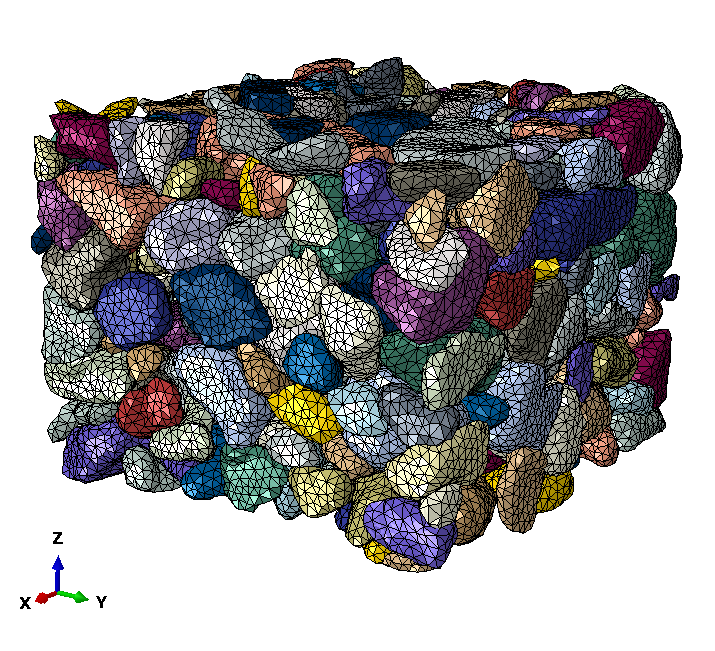
\includegraphics[width=\textwidth]{sample_after.png}
	\caption{\label{fig06:volume_simu_apres}\'Etat final de compression dans un sous-volume simulé. L'état initial est présenté sur la figure \ref{fig05:assemblage_abaqus}. Les déformations et contraintes moyennées dans ce volume sont les déformations et contraintes dites mésoscopiques.}
\end{figure}
	\subsection{Tenseur des déformations}\label{para06:green_lagrange}
		Le champ de déformation du volume numérique est calculé par une méthode de minimisation par les moindres carrés appliqués aux vecteurs déplacement de chaque grain. L'annexe \ref{annexe:deformations} explique en détail la méthode utilisée. L'idée est de considérer chaque grain numérisé par la position et le déplacement de son centre de masse au cours du temps. La méthode des moindres carrés est ainsi mise en \oe{}uvre pour estimer le tenseur gradient des déplacements $\doubleunderline{H}$. \`A partir du tenseur $\doubleunderline{H}$, il est possible de déterminer le tenseur des déformations de Green-Lagrange $\doubleunderline{E}$ qui tient compte des grandes déformations grâce au terme quadratique qui apparaît dans la formule (\ref{eq06:E_H}) :
		\begin{equation}\label{eq06:E_H}
			\doubleunderline{E}
			= \cfrac{1}{2}\left( \doubleunderline{H} + \doubleunderline{H}^T + \doubleunderline{H}^T \doubleunderline{H} \right)
		\end{equation}
		Le tenseur $\doubleunderline{H}$ s'exprime en fonction des vecteurs déplacement $\underline{u}$ et position $\underline{x}$ associés aux points matériels du milieu par la relation (\ref{eq06:H_u-x}) :
		\begin{equation}\label{eq06:H_u-x}
			\underline{u}
			= \doubleunderline{H} \cdot \underline{x} + \underline{u^0}
		\end{equation}
		où $\underline{u^0}$ est le vecteur déplacement moyen, associé au déplacement de corps rigide. L'équation (\ref{eq06:H_u-x}) peut se réécrire sous la forme modifiée suivante :
		\begin{equation}\label{eq06:H_u-x_modifie}
			\underline{\tilde{u}}
			= \doubleunderline{\tilde{H}} \cdot \underline{\tilde{x}}
			\quad\text{avec}\quad
			\underline{\tilde{u}}
			= \begin{bmatrix}
			u_1\\u_2\\u_3\\1\end{bmatrix}
			\;\text{,}\quad
			\doubleunderline{\tilde{H}}
			= \begin{bmatrix}
			H_{11} & H_{12} & H_{13} & u_1^0\\
			H_{21} & H_{22} & H_{23} & u_2^0\\
			H_{31} & H_{32} & H_{33} & u_3^0\\
			u_1^0 & u_2^0 & u_3^0 & \tilde{H}_{44}
			\end{bmatrix}
			\;\text{et}\quad
			\underline{\tilde{x}}
			= \begin{bmatrix}
			x_1\\x_2\\x_3\\1\end{bmatrix}
		\end{equation}
		$\underline{\tilde{u}}$, $\doubleunderline{\tilde{H}}$ et $\underline{\tilde{x}}$ sont, respectivement, le vecteur déplacement modifié, le tenseur gradient des déplacements modifié et le vecteur position modifié.
		\\Pour un échantillon constitué de $N$ grains, et d'après (\ref{eq06:H_u-x_modifie}), il est possible d'estimer par une méthode des moindres carrés le tenseur $\doubleunderline{\tilde{H}}$ à partir de la connaissance des vecteurs déplacement modifié $\underline{\tilde{u}}^g$ et position modifié $\underline{\tilde{x}}^g$ de chacun des centres de masse des grains $g$ constituant le milieu. Il faut alors minimiser le terme défini par (\ref{eq06:chi_carre}) :
		\begin{equation}\label{eq06:chi_carre}
		\chi^2
		= \sum_{g=1}^{N} \lVert \doubleunderline{\tilde{H}} \cdot \underline{\tilde{x}}^g - \underline{\tilde{u}}^g \rVert^2
		\end{equation}
		Les calculs réalisés dans l'annexe \ref{annexe:deformations} montrent qu'à partir des matrices définies selon (\ref{eq06:def_A_B}) :
		\begin{equation}\label{eq06:def_A_B}
			\forall i,j = 1,2,3,4\quad\quad\left\{
			\begin{array}{l}
				A_{ij} = \sum\limits_{\alpha=1}^N \tilde{x}_i^\alpha \tilde{x}_j^\alpha\\\\
				B_{ij} = \sum\limits_{\alpha=1}^{N} \tilde{u}_i^\alpha \tilde{x}_j^\alpha
			\end{array}\right.
		\end{equation}
		il est possible d'estimer le tenseur gradient des déplacements modifié $\doubleunderline{\tilde{H}}$ par l'intermédiaire de l'équation (\ref{eq06:def_H_A-B}) :
		\begin{equation}\label{eq06:def_H_A-B}
			\doubleunderline{\tilde{H}} = \doubleunderline{B} \cdot \doubleunderline{A}^{-1}
		\end{equation}
		\`A partir de $\doubleunderline{\tilde{H}}$ il est possible de déterminer le tenseur gradient des déplacements $\doubleunderline{H}$ grâce à la relation (\ref{eq06:H_Htilde}) suivante.
		\begin{equation}\label{eq06:H_Htilde}
			\forall i,j = 1,2,3\qquad
			H_{ij} = \tilde{H}_{ij}
		\end{equation}
		Enfin, le tenseur des déformations est obtenu en utilisant la relation (\ref{eq06:H_Htilde}) dans (\ref{eq06:E_H}).
		\\La figure \ref{fig06:deformation moyenne} illustre la manière de calculer le tenseur de déformation moyen sur un échantillon 2D constitué de seulement trois grains. Pour rappel, l'ensemble des tâches numériques présentées dans ces travaux est réalisé sur des volumes constitués généralement de plusieurs centaines de grains.
		\begin{figure}\centering
			\begin{minipage}{0.49\textwidth}\centering
				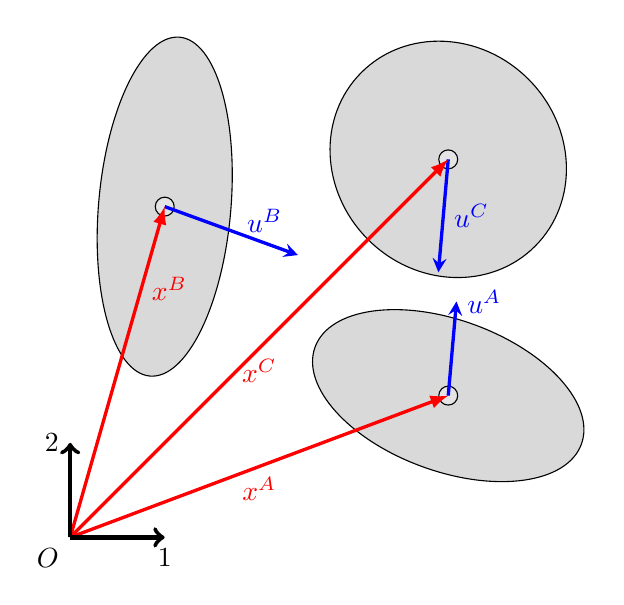
\begin{tikzpicture}[scale=1.2]
					% dessine trois particules
					\coordinate (A) at (4,1.5);
					\coordinate (B) at (1,3.5);
					\coordinate (C) at (4,4);
					\draw[fill=gray!30, rotate=-20] (A) ellipse (1.5 and 0.8);
					\draw[fill=gray!30, rotate=85] (B) ellipse (1.8 and 0.7);
					\draw[fill=gray!30, rotate=-45] (C) ellipse (1.3 and 1.2);
					% dessine les centres de masse
					\draw[fill=white, fill opacity=0.3] (A) circle (0.1);
					\draw[fill=white, fill opacity=0.3] (B) circle (0.1);
					\draw[fill=white, fill opacity=0.3] (C) circle (0.1);
					% dessine les déplacements
					\draw[very thick, blue, -stealth] (A) -- ++(85:1) node[right]{$\bm{u^A}$};
					\draw[very thick, blue, -stealth] (B) -- ++(-20:1.5) node[near end, above]{$\bm{u^B}$};
					\draw[very thick, blue, -stealth] (C) -- ++(-95:1.2) node[midway, right]{$\bm{u^C}$};
					% dessine les positions
					\draw[very thick, red, -latex] (0,0) -- (A) node[midway, below]{$\bm{x^A}$};
					\draw[very thick, red, -latex] (0,0) -- (B) node[near end, right]{$\bm{x^B}$};
					\draw[very thick, red, -latex] (0,0) -- (C) node[midway, below]{$\bm{x^C}$};
					% dessine le repère
					\draw[ultra thick, ->] (0,0) node[below left]{$O$} -- ++(1,0) node[below]{$1$};
					\draw[ultra thick, ->] (0,0) -- ++(0,1) node[left]{$2$};
				\end{tikzpicture}
			\end{minipage}
			\begin{minipage}{0.49\textwidth}\centering
				$$ A_{11} = {x_1^A}^2 + {x_1^B}^2 + {x_1^C}^2 $$
				$$ A_{22} = {x_2^A}^2 + {x_2^B}^2 + {x_2^C}^2 $$
				$$ A_{12} = A_{21} = x_1^Ax_2^A + x_1^Bx_2^B + x_1^Cx_2^C $$
				$$ B_{11} = u_1^Ax_1^A + u_1^Bx_1^B + u_1^Cx_1^C $$
				$$ B_{22} = u_2^Ax_2^A + u_2^Bx_2^B + u_2^Cx_2^C $$
				$$ B_{12} = u_1^Ax_2^A + u_1^Bx_2^B + u_1^Cx_2^C $$
				$$ B_{21} = u_2^Ax_1^A + u_2^Bx_1^B + u_2^Cx_1^C $$
			\end{minipage}
			\caption{\label{fig06:deformation moyenne}Schématisation 2D du principe de calcul de la déformation moyenne de l'échantillon numérique. La connaissance des vecteurs position (en rouge) et déplacement (en bleu) des centres de masse des particules permet de calculer les matrices $\doubleunderline{A}$ et $\doubleunderline{B}$ de la manière indiquée à droite de la figure.}
		\end{figure}
	\subsection{Tenseur des contraintes}\label{para06:love_weber}
		De la même manière que le tenseur des déformations mésoscopiques est calculé à partir de la connaissance des données cinématiques en un certain nombre de points, le tenseur des contraintes mésoscopiques est calculé à partir de la connaissance de forces exercées en un certain nombre de points dans le volume considéré. Le principe utilisé pour la définition du tenseur de contrainte est de faire une moyenne volumique des contraintes dans l'échantillon. Dans le formalisme des éléments finis, une manière simple de le faire consiste à calculer la moyenne des contraintes dans tous les éléments finis du modèle. Cependant, ceci implique de sauvegarder les valeurs de contrainte à tous les points d'intégration, ce qui représente une très grande quantité de données. Dans ce travail, les contraintes sont calculées à partir des forces de contact, ce qui permet de limiter considérablement la quantité de données à sauvegarder et simplifie  grandement le post-traitement et la gestion de l'espace disque.
		\begin{figure}\centering
			\begin{minipage}{0.44\textwidth}\centering
				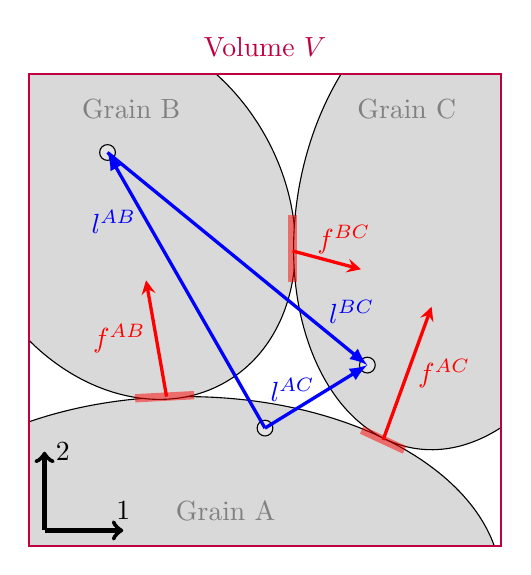
\begin{tikzpicture}[scale=1.]
				% dessine les grains
				\coordinate (A) at (2,-0.5);
				\coordinate (B) at (1.25,4.25);
				\coordinate (C) at (5.4,4.2);
				\begin{scope}
				\clip (0,0) rectangle (6,6);
				\draw[fill=gray!30] (A) ellipse (4 and 2.4);
				\draw[fill=gray!30, rotate=-60] (B) ellipse (2.5 and 2.);
				\draw[fill=gray!30, rotate=80] (C) ellipse (3 and 2.);
				\end{scope}
				\draw [gray] (2.5,0.2) node[above] {Grain A};
				\draw [gray] (1.3,5.8) node[below] {Grain B};
				\draw [gray] (4.8,5.8) node[below] {Grain C};
				% dessine les vecteurs entre grains
				\coordinate (Ap) at (3,1.5);
				\coordinate (Bp) at (1,5);
				\coordinate (Cp) at (4.3,2.3);
				\draw[fill=white, fill opacity=0.3] (Ap) circle (0.1);
				\draw[fill=white, fill opacity=0.3] (Bp) circle (0.1);
				\draw[fill=white, fill opacity=0.3] (Cp) circle (0.1);
				\draw[-latex, blue, very thick] (Ap) -- (Bp) node[near end, left] {$\bm{l^{AB}}$};
				\draw[-latex, blue, very thick] (Ap) -- (Cp) node[midway, above, xshift=-0.3cm, yshift=-0.2cm] {$\bm{l^{AC}}$};
				\draw[-latex, blue, very thick] (Bp) -- (Cp) node[near end, right, xshift=0.2cm] {$\bm{l^{BC}}$};
				% dessine les zones et forces de contact
				\coordinate (AB) at (1.75,1.9);
				\coordinate (AC) at (4.5,1.35);
				\coordinate (BC) at (3.35,3.75);
				\draw[red, line width=3pt, opacity=0.5] (AB) -- ++(3:0.35);
				\draw[red, line width=3pt, opacity=0.5] (AB) -- ++(183:0.4);
				\draw[-stealth, red, very thick] (AB) -- ++(100:1.5) node[midway, left] {$\bm{f^{AB}}$};
				\draw[red, line width=3pt, opacity=0.5] (AC) -- ++(-25:0.3);
				\draw[red, line width=3pt, opacity=0.5] (AC) -- ++(180-25:0.3);
				\draw[-stealth, red, very thick] (AC) -- ++(70:1.8) node[midway, right] {$\bm{f^{AC}}$};
				\draw[red, line width=3pt, opacity=0.5] (BC) -- ++(90:0.45);
				\draw[red, line width=3pt, opacity=0.5] (BC) -- ++(180+90:0.4);
				\draw[-stealth, red, very thick] (BC) -- ++(-15:0.9) node[near end, above] {$\bm{f^{BC}}$};
				% dessine le repère
				\draw[ultra thick, ->] (0.2,0.2) -- ++(1,0) node[above]{$1$};
				\draw[ultra thick, ->] (0.2,0.2) -- ++(0,1) node[right]{$2$};
				% dessine le volume
				\draw[purple, thick] (0,0) rectangle (6,6);
				\draw[purple] (3,6.1) node[above]{Volume $V$};
				\end{tikzpicture}
			\end{minipage}
			\begin{minipage}{0.55\textwidth}\centering
				$$ \overline{\sigma_{11}} = \left( f_1^{AB}l_1^{AB} + f_1^{AC}l_1^{AC} + f_1^{BC}l_1^{BC} \right)/V $$
				$$ \overline{\sigma_{22}} = \left( f_2^{AB}l_2^{AB} + f_2^{AC}l_2^{AC} + f_2^{BC}l_2^{BC} \right)/V $$
				$$ \overline{\sigma_{12}} = \overline{\sigma_{21}} = \left( f_1^{AB}l_2^{AB} + f_1^{AC}l_2^{AC} + f_1^{BC}l_2^{BC} \right)/V $$
			\end{minipage}
			\caption{\label{fig06:contrainte_moyenne}Schématisation 2D du principe de calcul de la contrainte moyenne dans l'échantillon numérique. La connaissance des efforts de contact (en rouge) et la position des grains entre eux (en bleu) permet de calculer un tenseur de contrainte de la manière indiquée à droite de la figure.}
		\end{figure}
		\\L'annexe \ref{annexe:contraintes} présente les détails du calcul du tenseur moyen des contraintes dans le volume et la figure \ref{fig06:contrainte_moyenne} permet de visualiser les différents éléments participant à ce calcul.
		\\Considérons un volume $V$ à l'équilibre statique dans lequel plusieurs particules sont en contact. Soit désormais $n$ le nombre de contacts qu'il existe au sein de ce même volume $V$ entre les particules. Pour deux particules en contact ($\alpha$ et $\beta$), va être défini :
		\begin{itemize}
			\item une force de contact ponctuelle unique $\bm{f^{\alpha\beta}}$ associée à la réponse du grain $\beta$ sur le grain $\alpha$ au niveau du point de contact\footnote{En théorie le contact n'est pas ponctuel mais on peut montrer (cf. annexe \ref{annexe:contraintes}) que la contrainte ne dépend que de la force résultante des efforts de contact et non de leur moment.}.
			\item un vecteur intergranulaire $\bm{l^{\alpha\beta}}$ qui relie un point quelconque du grain $\alpha$ à un un point quelconque du grain $\beta$. Le point associé à la particule peut être choisi arbitrairement mais il doit être unique : si la particule $\beta$ est également en contact avec une particule $\gamma$ alors le vecteur $\bm{l^{\beta\gamma}}$ doit être porté par le même point que celui qui reçoit le vecteur $\bm{l^{\alpha\beta}}$.
		\end{itemize}
		Les travaux de \citet{love_treatise_1927} et \citet{weber_recherches_1966} ont permis d'établir une contrainte moyenne $\overline{\sigma}$ dans un milieu granulaire, comme décrit dans les paragraphes précédents, par l'intermédiaire des relations (\ref{eq06:love_weber}) :
		\begin{equation}\label{eq06:love_weber}
			\overline{\sigma_{ij}}
			= \cfrac{1}{V} \sum_{\alpha\beta=1}^{n} f_i^{\alpha\beta} l_j^{\alpha\beta}
		\end{equation}
		Le tenseur des contraintes ainsi formulé par Love et Weber sera celui qui décrira l'état de chargement du volume numérique dans son intégralité. Ce tenseur est calculé pour chaque incrément de chargement en tenant compte de la variation du volume mésoscopique $V$ grâce à la connaissance du tenseur gradient de la transformation $\doubleunderline{F}$ calculé de la manière indiquée dans le paragraphe \ref{para06:green_lagrange}. Si $V_0$ est le volume mésoscopique avant chargement alors $V$ est défini par : $V = V_0 \times \mathrm{det}(\doubleunderline{F})$.
		
\section{Comparaison des champs cinématiques}\label{para06:comparaison_defo}
	Le travail expérimental qui consiste à procéder à la compression triaxiale d'un milieu granulaire et, dans le même temps, de procéder à l'imagerie 3D couplée à de la corrélation de volumes rend possible l'analyse des champs de déplacement et de déformation au sein de l'échantillon (cf. paragraphe \ref{para04:cinematique}). Les simulations permettent également de mesurer, par l'intermédiaire de la méthode décrite dans le paragraphe \ref{para06:green_lagrange}, les déformations du volume soumis à la simulation. Une comparaison des déformations mesurées sur les volumes numériques et sur les mêmes volumes issus de la corrélation d'images est nécessaire afin de vérifier la cohérence des conditions aux limites appliquées pour la simulation. Pour bien préciser cette approche, il est à noter que, comme expliqué au chapitre \ref{chap:numerique}, les déplacements mesurés par corrélation de volumes sont imposés à la simulation. Mais ils ne sont imposés qu'aux grains situées en périphérie du volume de contrôle, et pas sur tous les degrés de libertés. La comparaison effectuée ci-après est effectuée sur la déformation calculée d'après les déplacements de l'ensemble des grains du volume de contrôle. Cette déformation n'est pas nécessairement la même que celle qu'on obtient en ne considérant que les grains pilotés, et ce, autant dans les simulations numériques que dans les mesures de corrélation de volumes. Autrement dit, cette étape cherche à vérifier dans quelle mesure la cinématique des grains non pilotés dans la simulation est comparable à celle du même ensemble de grains dans l'expérience. Le paragraphe ci-dessous explique la manière dont a été calculée la déformation sur l’échantillon réel scanné par imagerie 3D.
	\subsection{Calcul de la déformation du sous-volume de l'échantillon}
		Afin de considérer la même définition de la déformation mésoscopique sur le volume décrit par l'imagerie 3D, la procédure de calcul est la même que pour le volume issu de la simulation par la méthode MP-FEM. Alors que pour le volume simulé les déplacements connus sont ceux des centres de masse, en ce qui concerne le volume issu de l'imagerie les déplacements connus sont situés aux centres des imagettes utilisées lors de la corrélation de volume, ces points sont appelés n\oe{}uds de corrélation par la suite. La connaissance des positions et déplacements des n\oe{}uds de corrélation au sein du volume concerné permet de générer les matrices $\doubleunderline{A}^C$ et $\doubleunderline{B}^C$ définies de la même manière qu'au paragraphe \ref{para06:green_lagrange}. Ces matrices sont ensuite utilisées pour déterminer un tenseur des déformations de Green-Lagrange par l'intermédiaire des équations (\ref{eq06:def_H_A-B}), (\ref{eq06:H_Htilde}) et (\ref{eq06:E_H}).
		\begin{figure}\centering
			\begin{minipage}{0.44\textwidth}\centering
				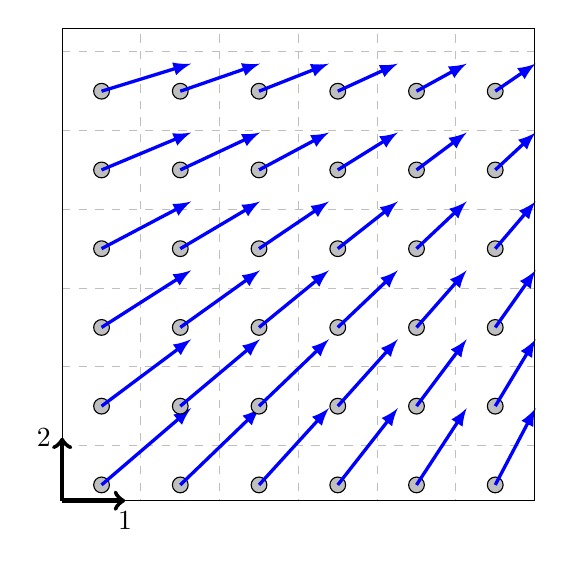
\begin{tikzpicture}[scale=1.]
				% dessine les imagettes
				\begin{scope}
				\clip (0,0) rectangle (6,6);
				\draw [gray!50, dashed, yshift=-.3cm] (0,0) grid[step=1] (6,7);
				\end{scope}
				% dessine les noeuds de corrélation et les déplacements
				\foreach \x in {0.5,1.5,...,5.5} {
					\foreach \y in {0.2,1.2,...,5.2} {
						\filldraw [fill=gray!50] (\x,\y) circle (0.1);
						\draw[blue, very thick, -latex] (\x,\y) -- ++(1.2-\x/8,1-\y/8);
					}
				}
				% dessine le cadre
				\draw (0,0) rectangle (6,6);
				% dessine le repère
				\draw[ultra thick, ->] (0,0) -- ++(0.8,0) node[below]{$1$};
				\draw[ultra thick, ->] (0,0) -- ++(0,0.8) node[left]{$2$};
				\end{tikzpicture}
			\end{minipage}
			\begin{minipage}{.55\textwidth}
				Pour un volume issu des résultats de corrélation contenant $N$ n\oe{}uds :
				$$ \forall i,j = 1,2,3,4 $$
				$$
				A_{ij}^C = \sum_{n=1}^{N} \tilde{x}_i^n\tilde{x}_j^n
				\quad\text{et}\quad
				B_{ij}^C = \sum_{n=1}^{N} \tilde{u}_i^n\tilde{x}_j^n
				$$
				où les $\tilde{x}_i^n$ et les $\tilde{u}_i^n$ sont respectivement les vecteurs modifiés position et déplacement du n\oe{}uds $n$.
			\end{minipage}
			\caption{\label{fig06:deformation_moyenne_DVC}Schématisation 2D du principe de calcul de la déformation moyenne du volume issu de l'échantillon réel à partir des positions (cercles gris) et déplacements (flèches bleues) des fenêtres de corrélation (carrés en pointillés).}
		\end{figure}
		La figure \ref{fig06:deformation_moyenne_DVC} illustre la manière de calculer les déformations mésoscopiques dans l'échantillon issu de l'imagerie 3D grâce aux résultats de la corrélation au niveau du volume simulé. Pour les travaux menés dans cette thèse, la distance qui sépare chaque n\oe{}ud de corrélation suivant chaque direction de l'espace est de \SI{10}{\voxel}, soit \SI{90}{\micro\meter} ou légèrement plus que la moitié de la taille d'un grain moyen. Les données en position et déplacement qui servent à approximer le gradient des déplacements sont donc généralement plus nombreuses lors du calcul de la déformation moyenne à partir de la corrélation de volume que lors du calcul sur le volume issu de la simulation (une seule information par grain\footnote{Il s'agit d'un choix délibéré : tous les déplacements nodaux auraient également pu être utilisés.}).
		\\Comme il a été vu au chapitre \ref{chap:numerique}, les grains situés en bordure de l'échantillon numérique se voient attribuer un déplacement issu du calcul de corrélation de volumes. Néanmoins, il convient de rappeler que tous les autres grains ne sont pas pilotés. Ainsi, la première vérification des résultats du modèle numérique consiste à comparer la déformation du volume occupé par les grains non pilotés entre le calcul numérique et la mesure de champ. Pour des raisons de simplicité de mise en \oe{}uvre, la comparaison est effectuée non pas sur les grains non pilotés mais sur l'ensemble du volume simulé, incluant les grains pilotés et les grains non pilotés.
		\\Seuls les n\oe{}uds de corrélation pour lesquels le coefficient de corrélation normalisé (cf. paragraphe \ref{para03:DIC}) est supérieur à \num{0.99} sont considérés dans le calcul afin d'assurer la validité du champ de déplacement retenu en fin de procédure.
		\paragraph{}
		Les calculs de la déformation mésoscopique au sein de l'échantillon simulé et de l'échantillon issu de l'imagerie 3D sont basés sur la même méthode et peuvent être comparés l'un à l'autre. Cette comparaison va être effectuée dans la partie qui suit, avec l'objectif de déterminer le domaine de validité des conditions aux limites appliquées dans les calculs de simulation.
	\subsection{Comparaison des déformations mésoscopiques}
		La comparaison des déformations calculées dans les images 3D et lors de la simulation va être menée sur :
		\begin{itemize}
			\item la déformation axiale $\varepsilon_{a}$, composante du tenseur des déformations calculée suivant la direction du chargement axial ;
			\item la déformation déviatoire $\varepsilon_d$, définie selon l'équation (\ref{eq03:decomposition_defo_triax}) ;
			\item la déformation volumique $\varepsilon_v$, définie également par l'équation (\ref{eq03:decomposition_defo_triax}).
		\end{itemize}
		Les volumes sur lesquels la déformation mésoscopique est mesurée et comparée à celle issue de la corrélation d'images 3D sont ceux présents aux centres des échantillons scannés. Ainsi, la comparaison est effectuée sur un volume situé au centre de chaque échantillon expérimental, et l'influence de la dimension de ce volume est étudiée. La taille de la bordure dans l'échantillon numérisé, permettant de déterminer le nombre de grains à piloter, est également analysée dans les paragraphes qui suivent. Les propriétés mécaniques du matériau constitutif des grains dans les simulations sont présentées sur le tableau \ref{tab06:prop_meca_comparaison_defo} et ne varient pas entre les différents essais présentés dans cette partie. Il s’agit en premier temps de faire une étude de sensibilité des résultats au travers de trois effets potentiels : effet de la taille du volume simulé,	effet de la pression de confinement et effet de la zone de pilotage des grains.
		\begin{table}\centering
			\begin{tabular}{r@{\hspace{.05\textwidth}}rl}
				\hline
				Propriété mécanique & \multicolumn{2}{c}{Valeur} \\
				\hline
				module de Young & \num{2.9} & \si{\giga\pascal}\\
				Coefficient de Poisson & \num{0.38} & \\
				Limite élastique & \num{45} & \si{\mega\pascal}\\
				Module d'écrouissage & \num{8.35} & \si{\mega\pascal} \\
				Coefficient de friction & \num{0.5} & \\\hline
			\end{tabular}
			\caption{\label{tab06:prop_meca_comparaison_defo}Propriétés mécaniques utilisées dans la loi de comportement élasto-plastique des grains pour les simulations numériques présentées dans la partie \ref{para06:comparaison_defo}}
		\end{table}
		\subsubsection{Effet de la taille du volume simulé}
			L'objectif de ce paragraphe est d'étudier l'effet de la taille du sous-volume de l'échantillon qui est simulé sur la validité des conditions aux limites. Pour cela, la comparaison des déformations va être réalisée sur différents sous-volumes centrés au milieu de l'échantillon subissant une pression de confinement de \SI{2}{\mega\pascal}. Ces sous-volumes ont une forme cubique. Le plus petit sous-volume étudié a une longueur d'arête de \SI{540}{\micro\meter} et contient \num{87} grains tandis que le plus grand sous-volume étudié a une longueur d'arête de \SI{1.260}{\milli\meter} et contient 829 grains. Le nombre de grains sur la bordure du sous-volume augmente logiquement avec la taille du sous-volume. Puisque ce sont les grains présents sur une certaine épaisseur de la bordure qui sont pilotés en déplacement, l'augmentation de la taille des volumes simulés engendre l'augmentation du nombre de grains auxquels un déplacement est imposé. L'épaisseur de la zone de pilotage des grains est constante tout au long de l'étude de l'effet de la taille des sous-volumes et vaut \SI{63}{\micro\meter}, soit légèrement en dessous de la moitié d'un grain moyen.
			\begin{figure}\centering
				\subfloat[longueur d'arête : \SI{540}{\micro\meter}]{
					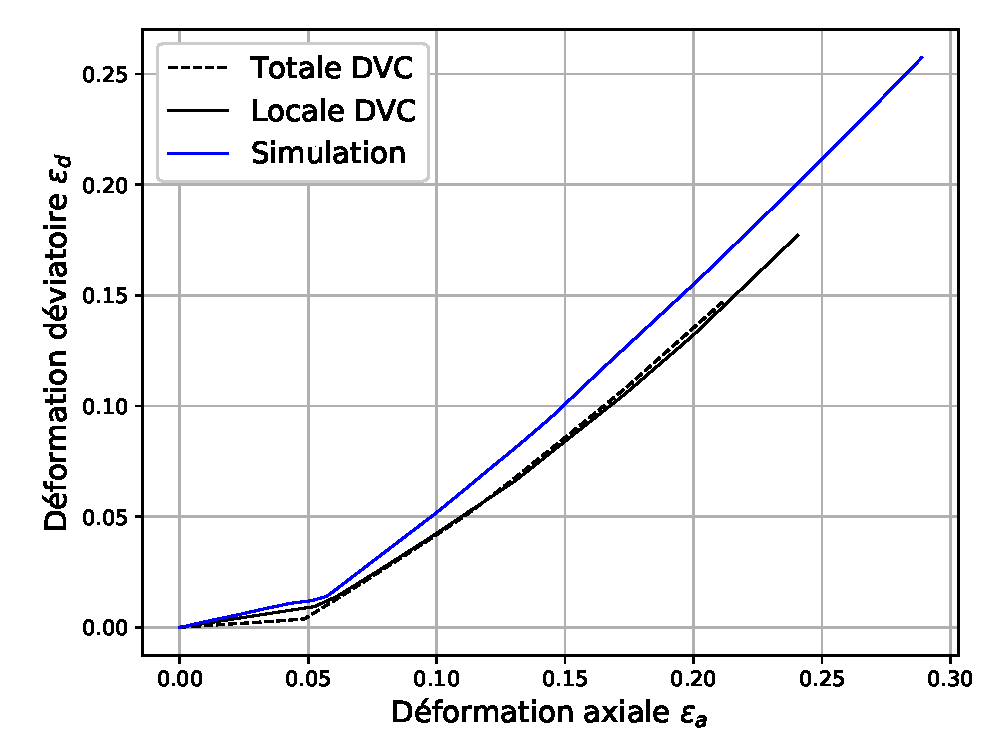
\includegraphics[width=.48\textwidth]{strains_box_size/060_deviatoire.eps}\hfill
					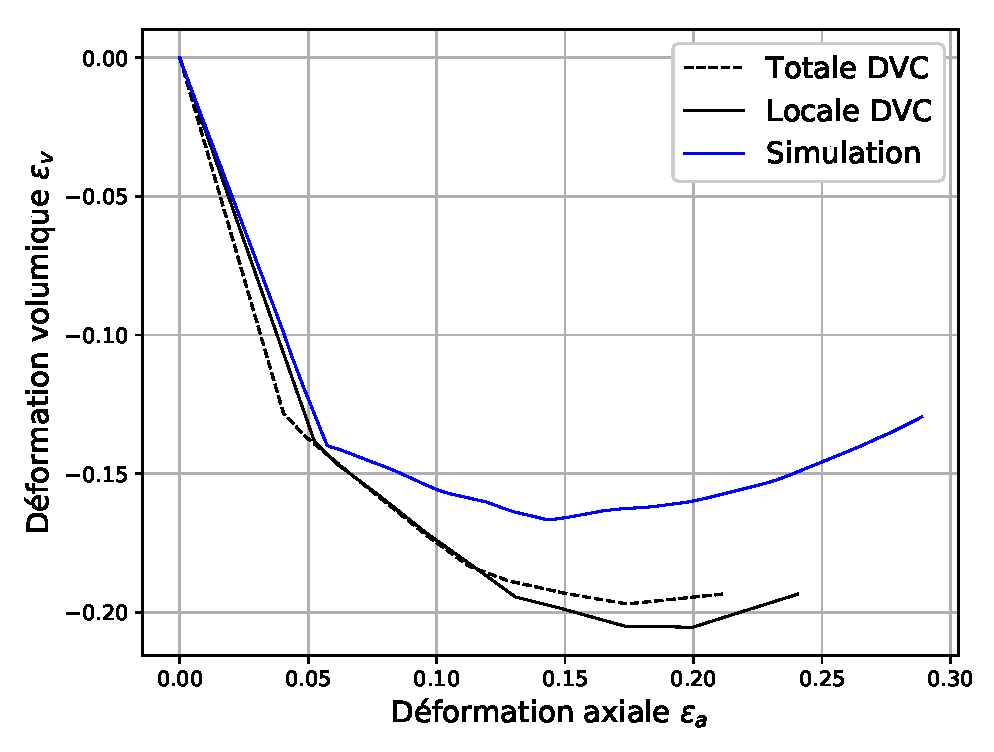
\includegraphics[width=.48\textwidth]{strains_box_size/060_volumique.eps}
				}\\
				\subfloat[longueur d'arête : \SI{810}{\micro\meter}]{
					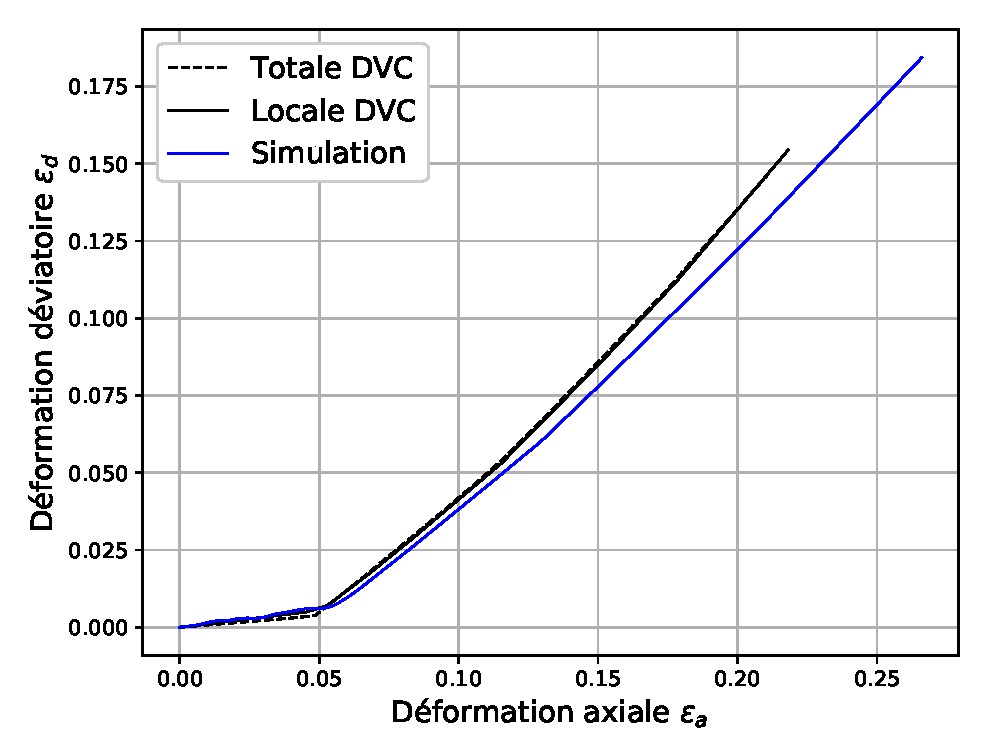
\includegraphics[width=.48\textwidth]{strains_box_size/090_deviatoire.eps}\hfill
					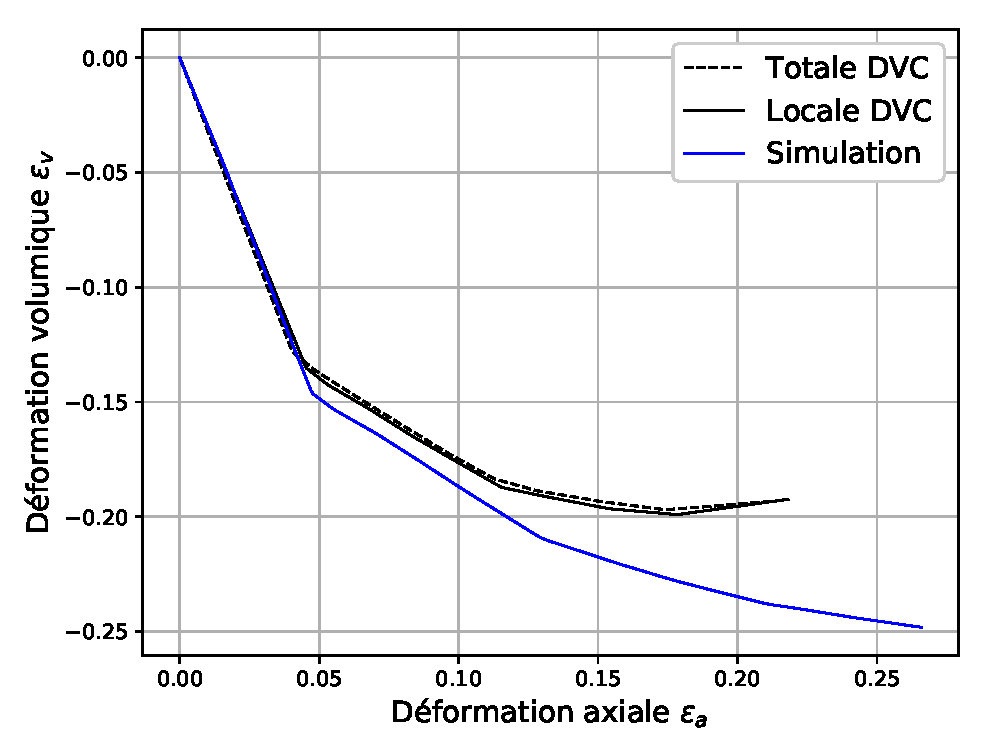
\includegraphics[width=.48\textwidth]{strains_box_size/090_volumique.eps}
				}\\
				\subfloat[longueur d'arête : \SI{1.260}{\milli\meter}]{
					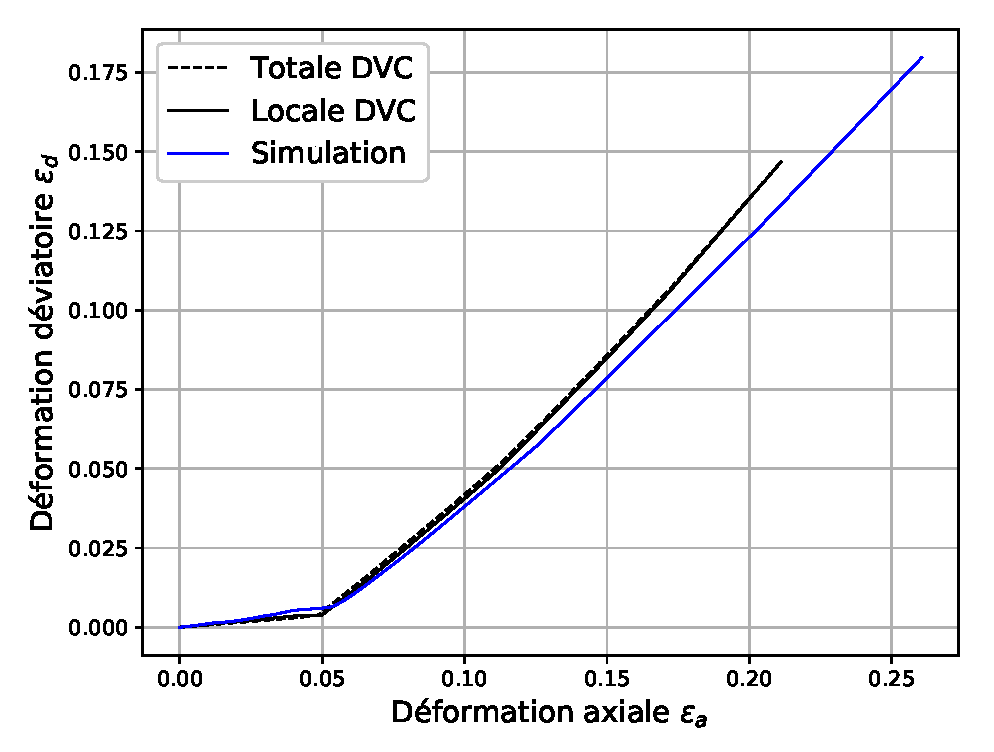
\includegraphics[width=.48\textwidth]{strains_box_size/140_deviatoire.eps}\hfill
					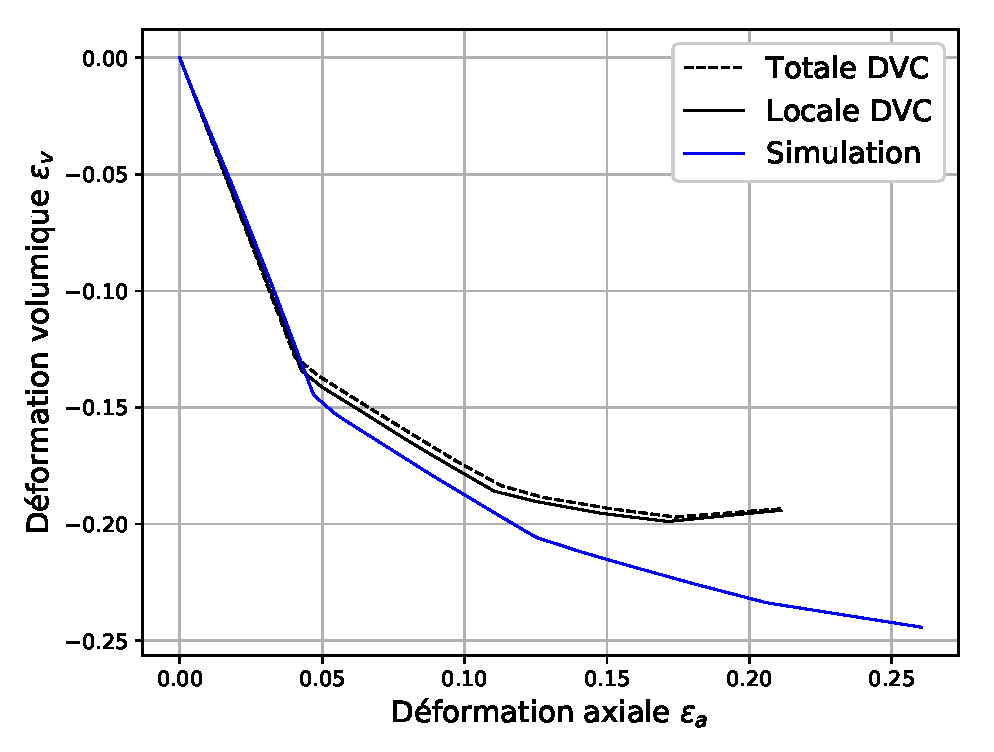
\includegraphics[width=.48\textwidth]{strains_box_size/140_volumique.eps}
				}
				\caption{\label{fig06:comparaison_defo_taille_volume}Déformations déviatoire (gauche) et volumique (droite) en fonction de la déformation axiale pour différentes tailles de sous-volumes. La courbe en trait pointillé noir correspond à la déformation moyenne de l'ensemble de l'échantillon mesurée par DVC ; en trait continu noir celle mesurée localement par DVC ; et en trait continu bleu celle mesurée localement dans la simulation.}
			\end{figure}
			\\L'évolution des déformations déviatoire et volumique en fonction de la déformation axiale est présentée sur la figure \ref{fig06:comparaison_defo_taille_volume}. Trois sous-volumes sont comparés : le plus petit dont la longueur d'arête est de \SI{540}{\micro\meter}, un sous-volume de taille moyenne avec une longueur d'arête de \SI{810}{\micro\meter} (contenant \num{253} grains) et le plus grand avec une longueur d'arête de \SI{1.260}{\milli\meter}. Sur ces graphes, l'évolution de la déformation mesurée par la simulation (courbe bleue continue) peut être comparée à celle de la déformation mesurée localement par la corrélation de volume (courbe noire continue). L'analyse de ces deux courbes concernant le plus petit des sous-volumes (figure \ref{fig06:comparaison_defo_taille_volume}-(a)) indique que la déformation moyenne calculée à partir de la simulation diffère rapidement de celle mesurée localement par la corrélation de volume. Lorsque la taille du volume simulé augmente (figure \ref{fig06:comparaison_defo_taille_volume}-(b) puis (c)), les déformations mésoscopiques calculées par corrélation et simulation sont sensiblement les mêmes pour les états de déformation faibles mais divergent au delà d'une déformation axiale d'environ \SI{10}{\percent}.
			\\Pour assurer des conditions aux limites quasi-identiques à celles observées sur l'échantillon réel, il est donc nécessaire de mener les simulations sur des volumes suffisamment grands. Dans ces travaux, la taille minimale du sous-volume permettant d'observer des conditions aux limites correctes est de telle sorte que la longueur d'arête du sous-volume soit de \num{5} à \num{6} fois la taille d'un grain moyen, de sorte à obtenir un volume constitué d'approximativement \num{250} grains. Les simulations menées sur des volumes plus grands ne semblent pas indiquer un rôle de la taille du volume dans l'évolution des déformations moyennes au delà de ce volume minimal. Il est à retenir également que l'évolution des déformations mésoscopiques obtenues par la simulation ne suit pas parfaitement celle des déformations calculées par corrélation pour les grands états de chargement.
		\subsubsection{Effet de la pression de confinement}
			Les sous-volumes de l'échantillon qui vont être simulés ont désormais une taille fixée, suffisamment grande pour considérer des conditions aux limites correctes. Le matériau constitutif des grains est toujours celui dont les propriétés sont présentées sur le tableau \ref{tab06:prop_meca_comparaison_defo}. La zone de pilotage des grains a une épaisseur qui ne varie pas pour le moment et vaut toujours \SI{63}{\micro\meter}. Dans ce paragraphe, seul l'effet de la pression de confinement et du chargement axial sur les conditions aux limites est observé. Pour ce faire, les sous-volumes pris au centres des différents échantillons sont considérés. L'hypothèse que la géométrie des grains intervient de la même manière pour chaque essai dans la réaction mécanique de l'échantillon est faite. Ainsi, seul le chemin de chargement évolue d'un échantillon à un autre.
			\begin{figure}\centering
				\subfloat[$P_C = \SI{1}{\mega\pascal}$]{
					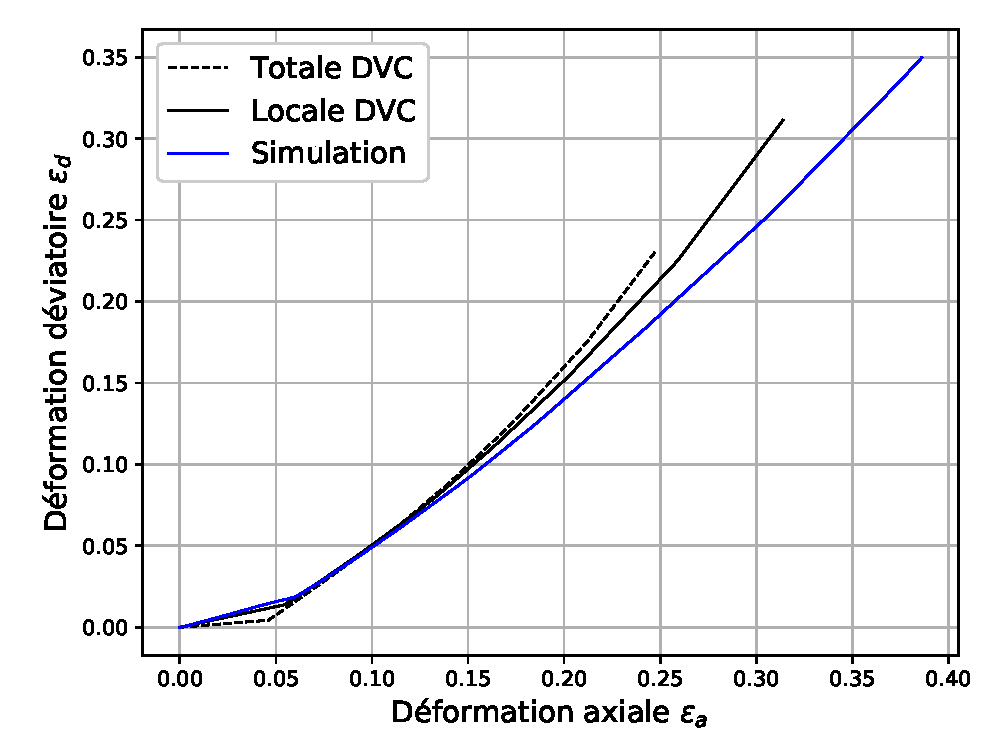
\includegraphics[width=.48\textwidth]{strains_loading/1_MPa_deviatoire.eps}\hfill
					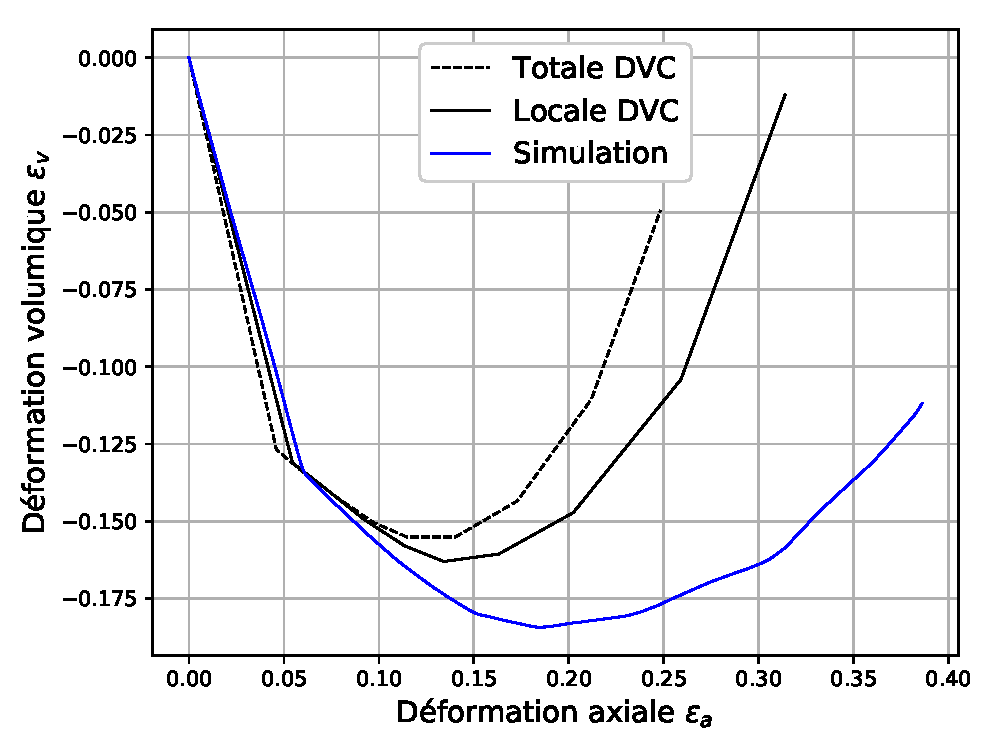
\includegraphics[width=.48\textwidth]{strains_loading/1_MPa_volumique.eps}\hfill
				}\\
				\subfloat[$P_C = \SI{2}{\mega\pascal}$]{
					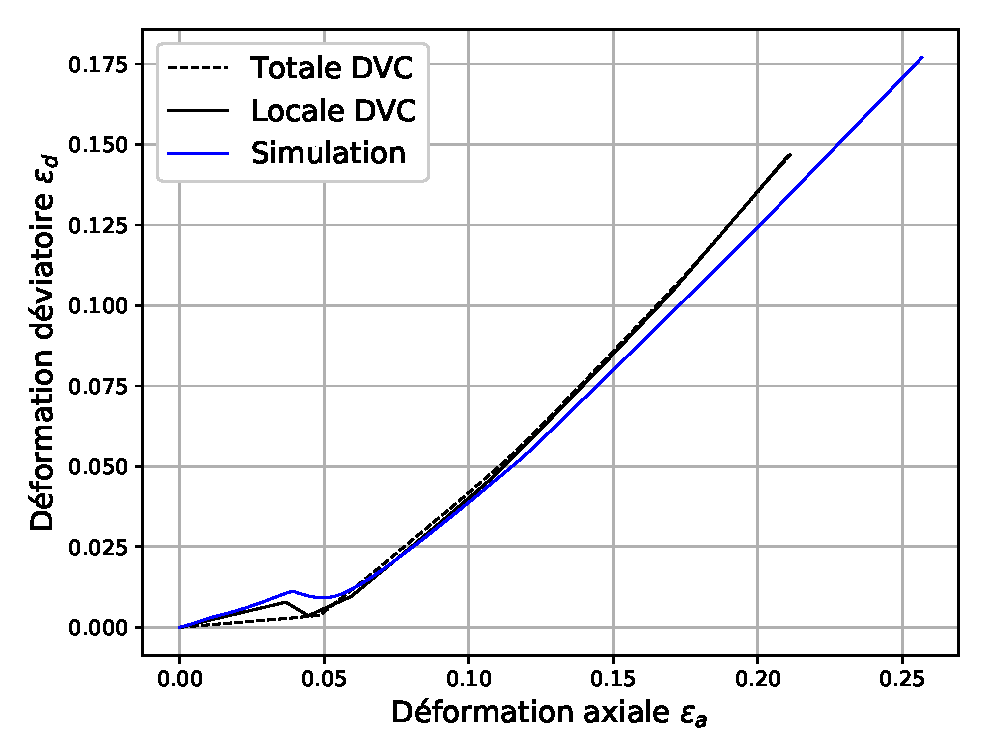
\includegraphics[width=.48\textwidth]{strains_loading/2_MPa_deviatoire.eps}\hfill
					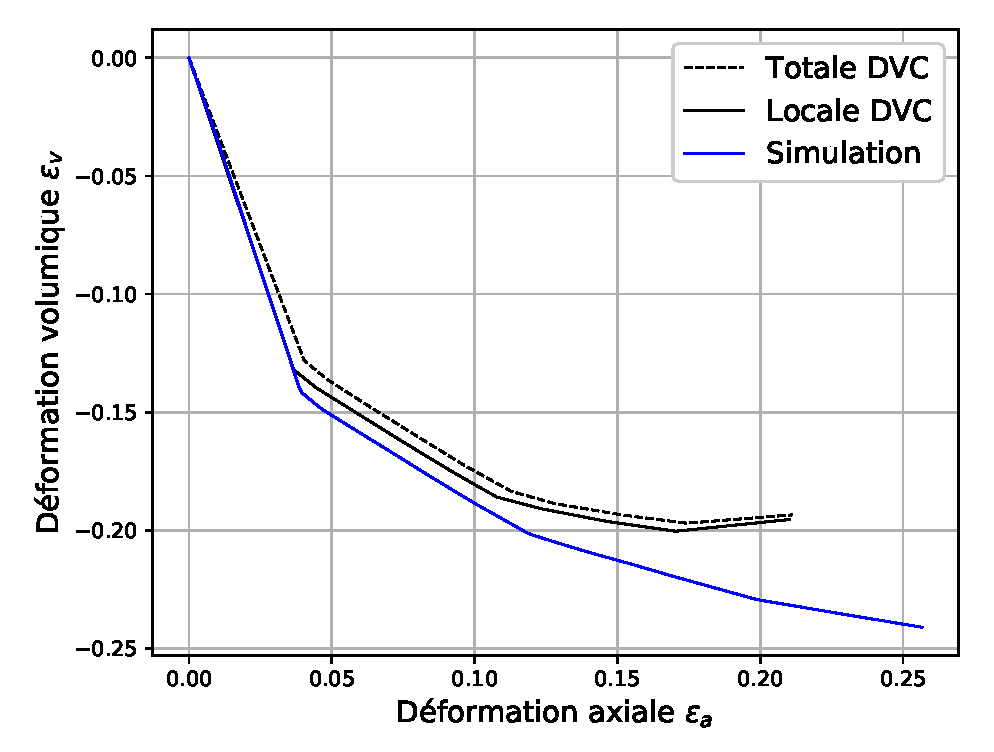
\includegraphics[width=.48\textwidth]{strains_loading/2_MPa_volumique.eps}\hfill
				}\\
				\subfloat[$P_C = \SI{7}{\mega\pascal}$]{
					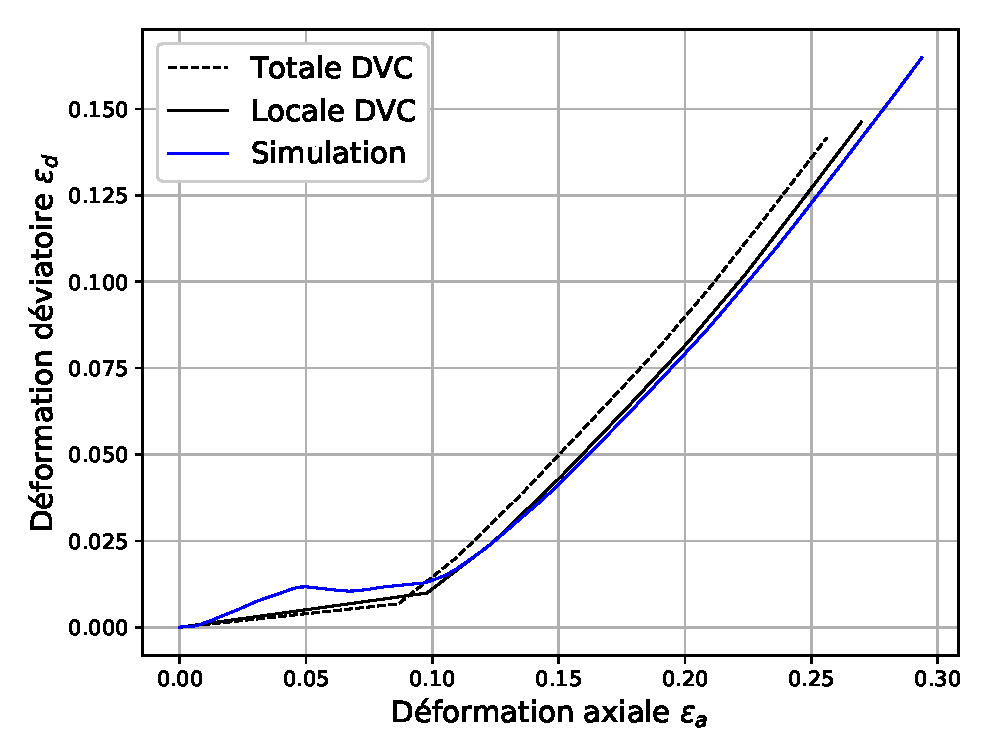
\includegraphics[width=.48\textwidth]{strains_loading/7_MPa_deviatoire.eps}\hfill
					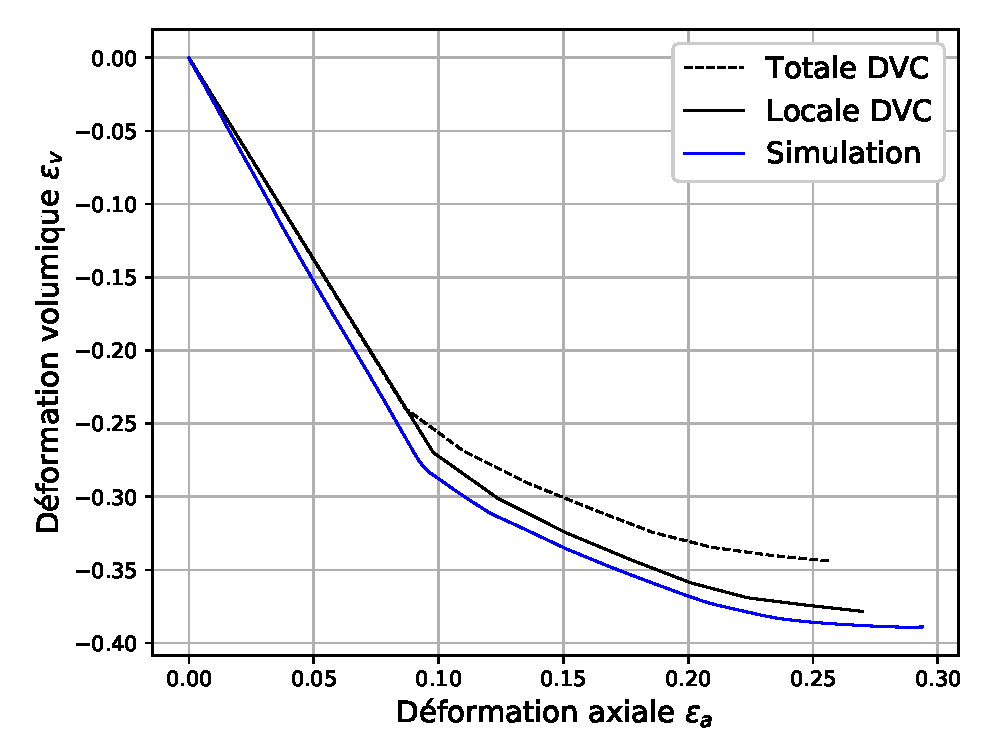
\includegraphics[width=.48\textwidth]{strains_loading/7_MPa_volumique.eps}\hfill
				}
				\caption{\label{fig06:comparaison_defo_chargement}Déformations déviatoire (gauche) et volumique (droite) en fonction de la déformation axiale pour différents chemins de chargement. La courbe en trait pointillé noir correspond à la déformation moyenne de l'ensemble de l'échantillon mesurée par DVC ; en trait continu noir celle mesurée localement par DVC ; et en trait continu bleu celle mesurée localement dans la simulation.}
			\end{figure}
		\\La figure \ref{fig06:comparaison_defo_chargement} présente les courbes de déformation pour chacun des échantillon, qui subissent donc trois chemins de chargement différents. L'évolution des déformations mésoscopiques calculées par la simulation et la corrélation présente des similitudes très marquées. Il est noté en premier lieu que pour la pression de confinement de \SI{1}{\mega\pascal} (figure \ref{fig06:comparaison_defo_chargement}-(a)), on observe un effet de dilatance marqué : la déformation volumique augmente lorsque la déformation axiale dépasse \num{0.15} - \num{0.20}. Cet effet de dilatance est à peine visible pour la pression de confinement de \SI{2}{\mega\pascal} (figure \ref{fig06:comparaison_defo_chargement}-(b)) et plus du tout à \SI{7}{\mega\pascal} (figure \ref{fig06:comparaison_defo_chargement}-(c)). On retrouve ici un effet connu pour les poudres à grains déformables : en effet la déformabilité des grains leur permet de subir un cisaillement sans imposer une augmentation du volume macroscopique. Un exemple de déformation de grain est donné sur la figure \ref{fig06:defo_grain} représentant la morphologie d'un grain pour différents états du chargement issu d'une simulation menée avec une pression de confinement de \SI{7}{\mega\pascal}. Ainsi, à \SI{1}{\mega\pascal}, la poudre de polystyrène se rapproche d'un milieu à grains rigides, à \SI{7}{\mega\pascal} la déformabilité des grains se fait sentir.
		\begin{figure}\centering
			~\hfill
			\subfloat[\'Etat initial]{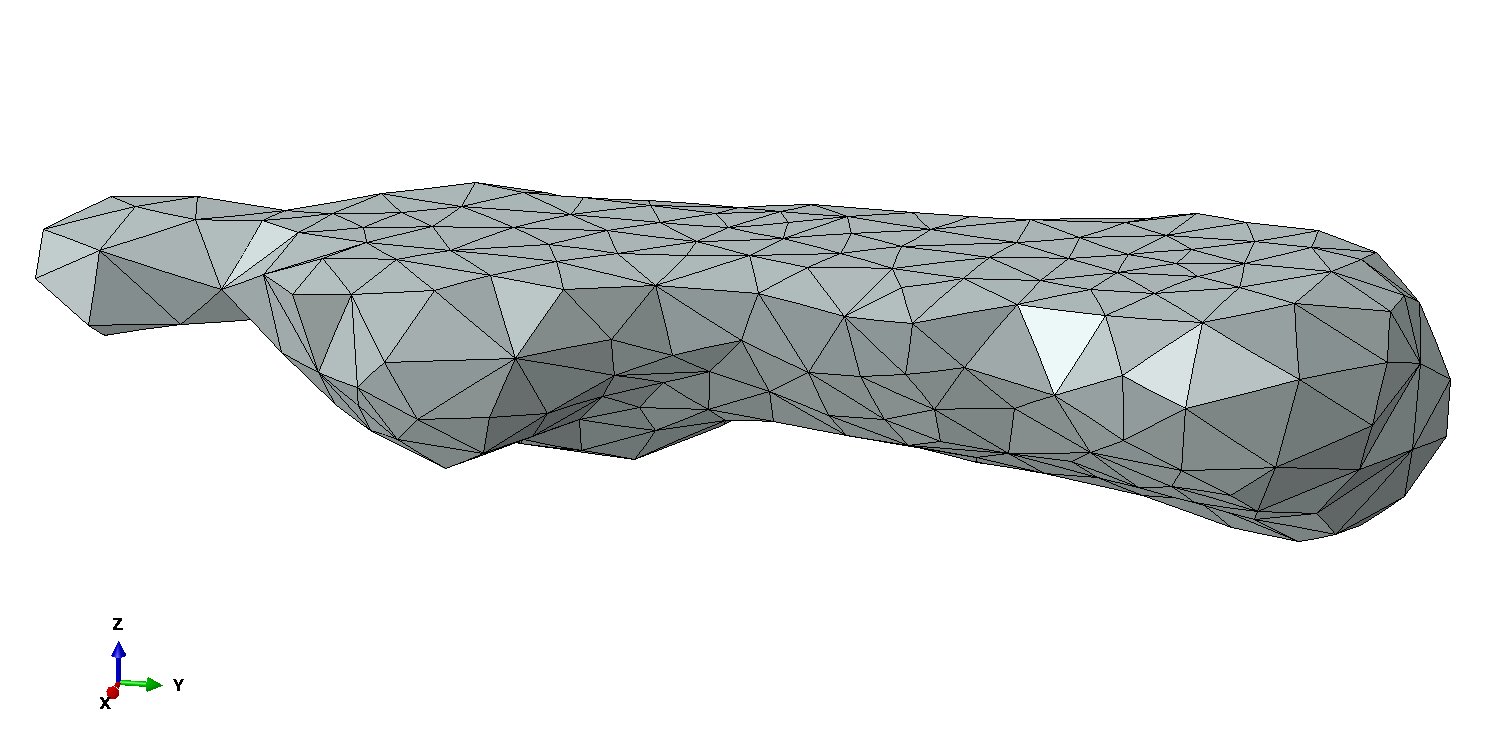
\includegraphics[width=.45\textwidth]{grain_deforme/grain_00}}\hfill
			\subfloat[Déformation axiale : \num{0.09}]{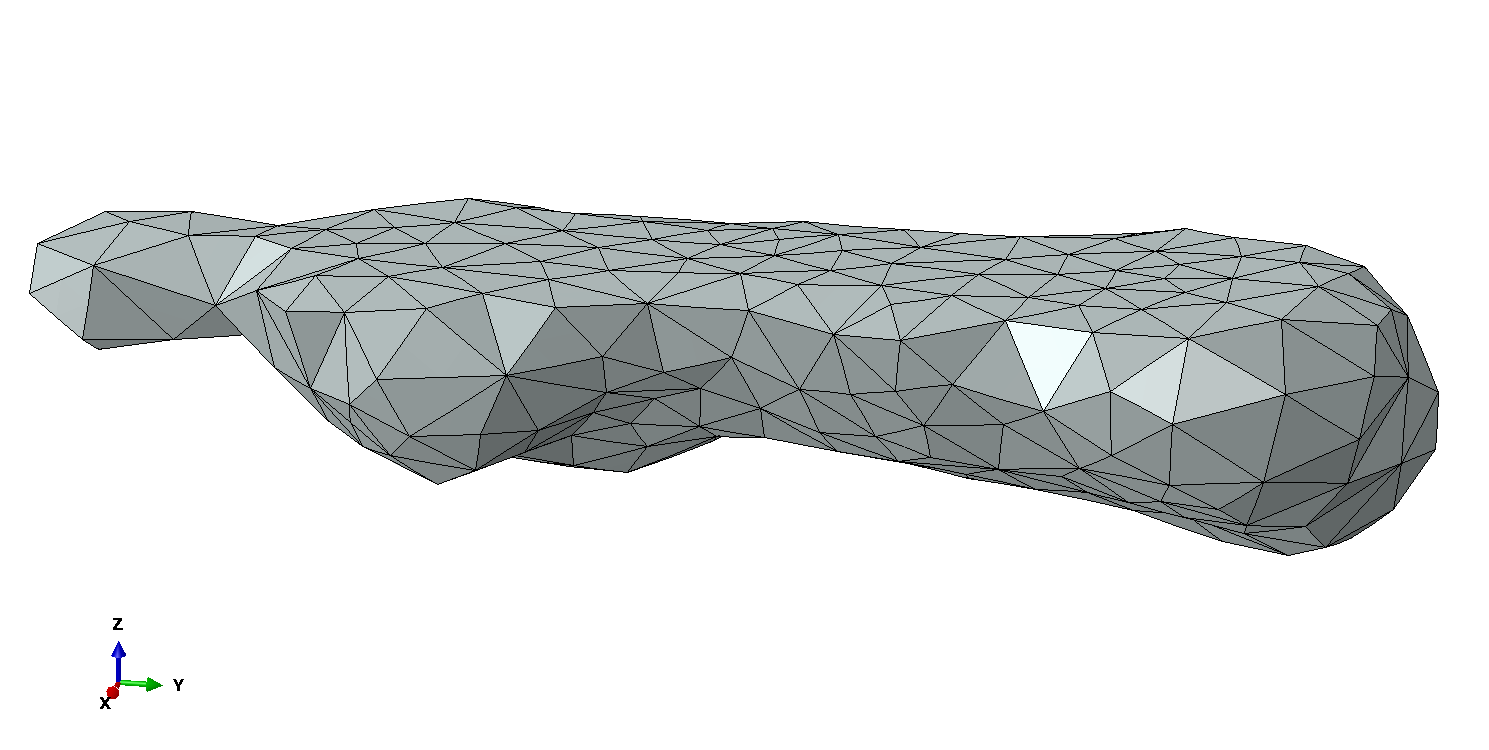
\includegraphics[width=.45\textwidth]{grain_deforme/grain_00_Pc}}
			\hfill~\\
			~\hfill
			\subfloat[Déformation axiale : \num{0.17}]{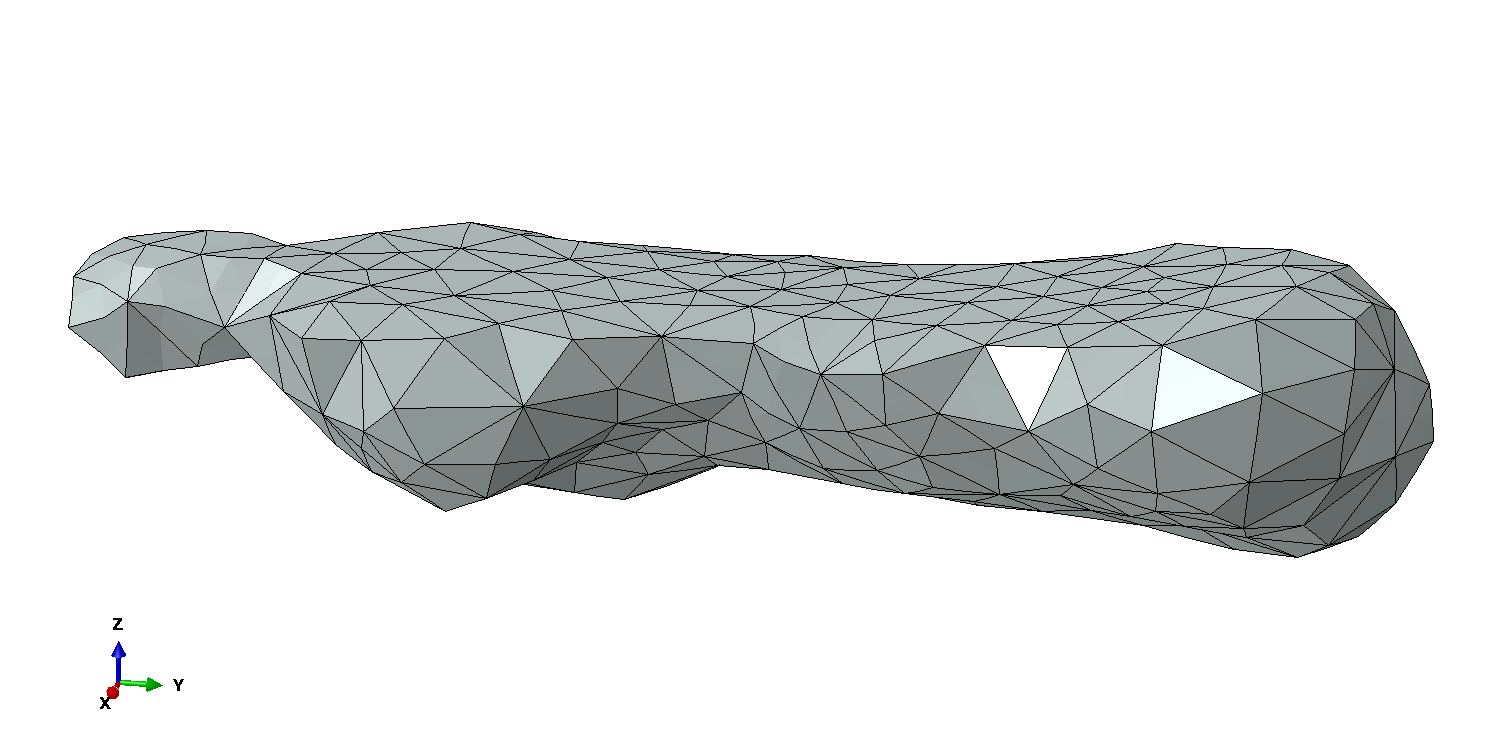
\includegraphics[width=.45\textwidth]{grain_deforme/grain_250}}\hfill
			\subfloat[Déformation axiale : \num{0.22}]{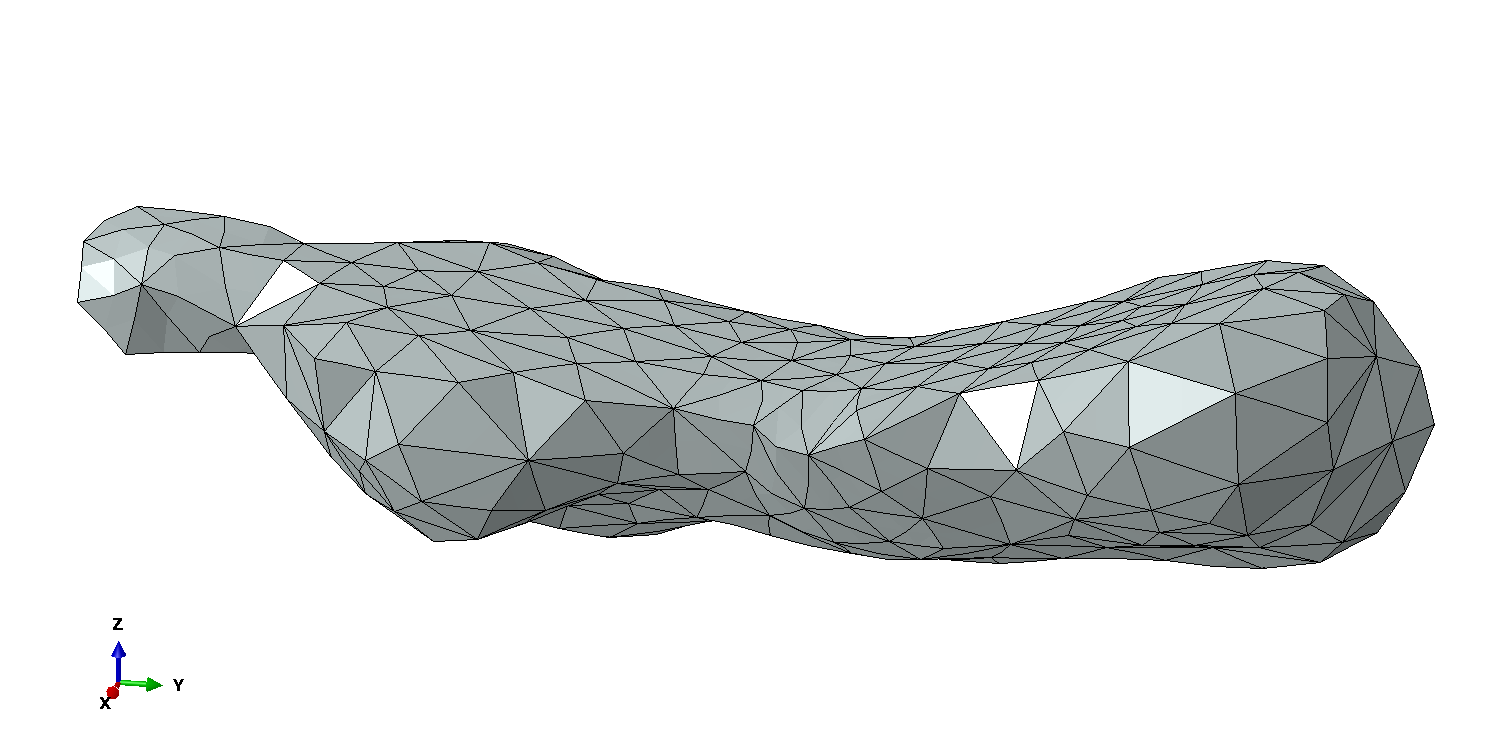
\includegraphics[width=.45\textwidth]{grain_deforme/grain_400}}
			\hfill~\\
			\subfloat[Déformation axiale : \num{0.28}]{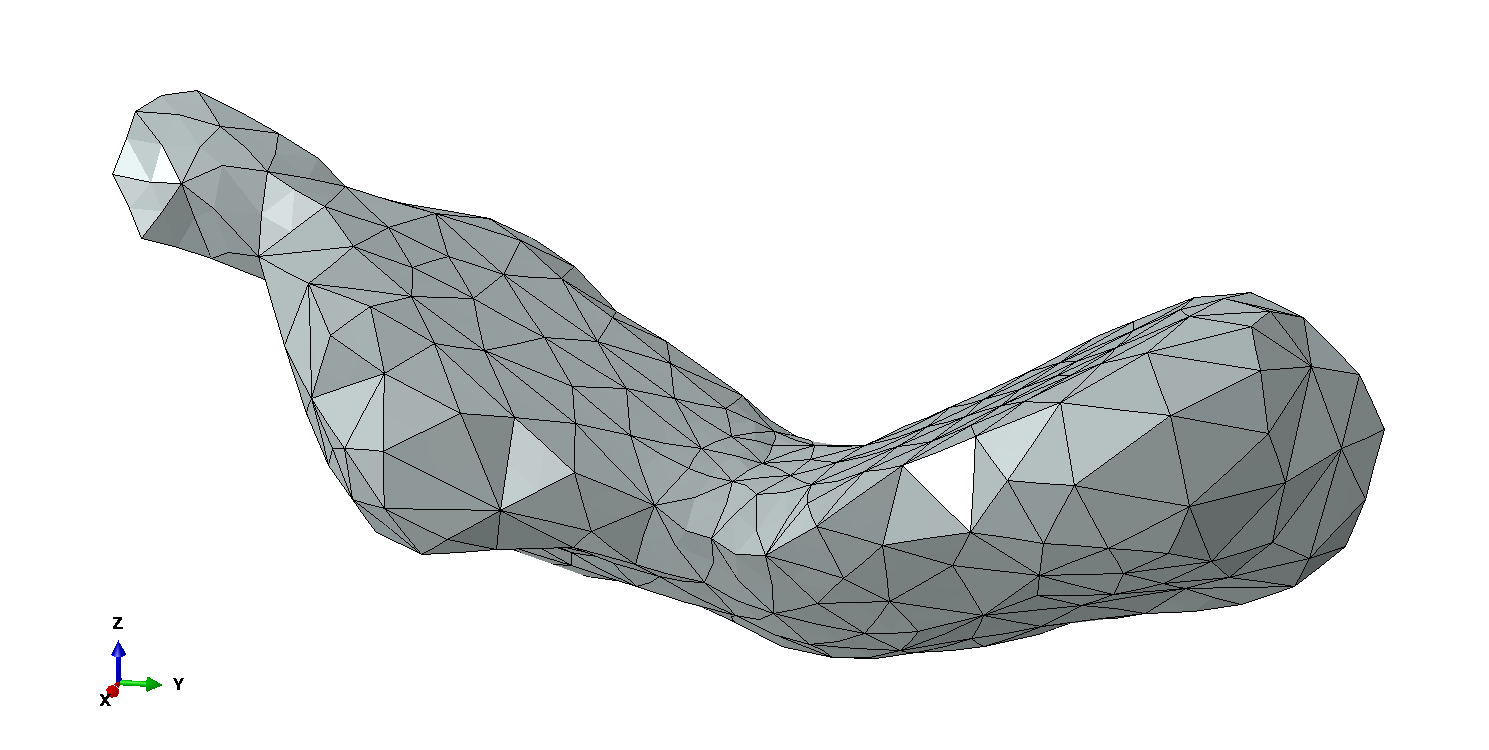
\includegraphics[width=.45\textwidth]{grain_deforme/grain_500}}
			\caption{\label{fig06:defo_grain}Déformation d'un grain issu d'une simulation avec une pression de confinement de \SI{7}{\mega\pascal} pour plusieurs états de chargement.}
		\end{figure}
		\\En étudiant l'ensemble des courbes présentées sur la figure \ref{fig06:comparaison_defo_chargement} ainsi que celles pour des sous-volumes situés à d'autres emplacements dans l'échantillon réel, il apparaît que la présence du phénomène de dilatance engendre une mauvaise évaluation du taux de densification, bien que l'effet soit observable. En effet, lors de la dilatance, l'amplitude de déplacement de certains grains est augmentée et le voisinage de chaque grain peut se retrouver significativement différent. Dans la simulation, seuls les grains initialement présents dans le sous-volume sont étudiés : si dans l'échantillon réel un grain non présent initialement dans le sous-volume étudié interagit avec les grains reconnus initialement alors la simulation n'en tiendra pas compte. Il est évident que cela aura également des conséquences sur le calcul de la contrainte moyenne dans l'échantillon puisque des forces de contact ne sont pas prises en compte. La validité des conditions aux limites dans la simulation numérique est donc sensible au chemin de chargement pour les grandes déformations. Toutefois, avant apparition de phénomènes liés à la dilatance les déformations sont similaires à celles observées dans l'échantillon réel.
		\subsubsection{Effet de la "zone de pilotage" des grains}
			Un autre paramètre très influent sur les conditions aux limites est l'épaisseur de la zone de pilotage des grains en périphérie du sous-volume. Pour rappel, cette zone correspond à une bordure de quelques voxels vers l'intérieur du sous-volume issu de la tomographie. Tous les grains qui se trouvent au moins en partie dans cette zone sont pilotés en déplacement, par l'intermédiaire des n\oe{}uds de référence placés aux centres de masse des grains pilotés (cf. paragraphe \ref{para05:abaqus_BC}). Afin d'analyser l'effet de cette zone de pilotage sur les conditions aux limites, plusieurs simulations sont réalisées sur un même sous-volume, en faisant varier l'épaisseur de la zone de pilotage des grains. Le matériau constitutif des grains est inchangé et correspond à celui décrit dans le tableau \ref{tab06:prop_meca_comparaison_defo}. Le volume simulé est un sous-volume centré dans l'échantillon dont la pression de confinement est de \SI{2}{\mega\pascal}. Le nombre de grains non pilotés en déplacement est constant (nombre de grains entiers dans un cube de \SI{900}{\micro\meter} de côté - équivalent à 6 grains moyens sur une arête) tandis que l'épaisseur de la zone de pilotage des grains autour varie entre \SI{45}{\micro\meter} et \SI{225}{\micro\meter}.
			\begin{figure}\centering
				\subfloat[Grains pilotés sur une bordure de \SI{45}{\micro\meter}]{
					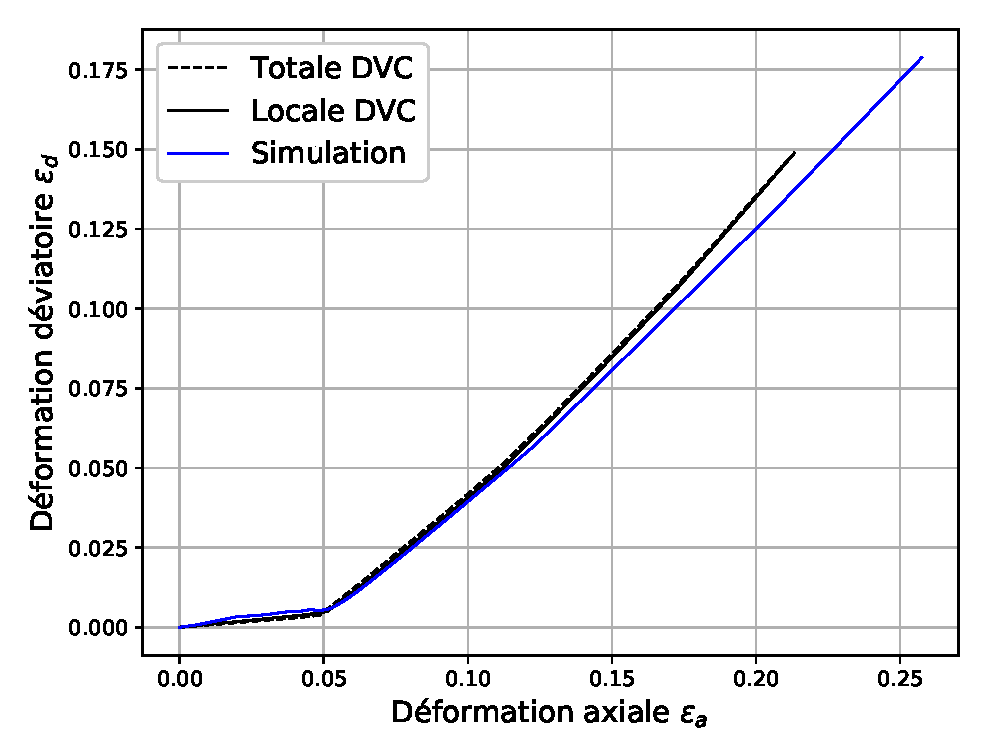
\includegraphics[width=.48\textwidth]{strains_border_size/005_deviatoire.eps}\hfill
					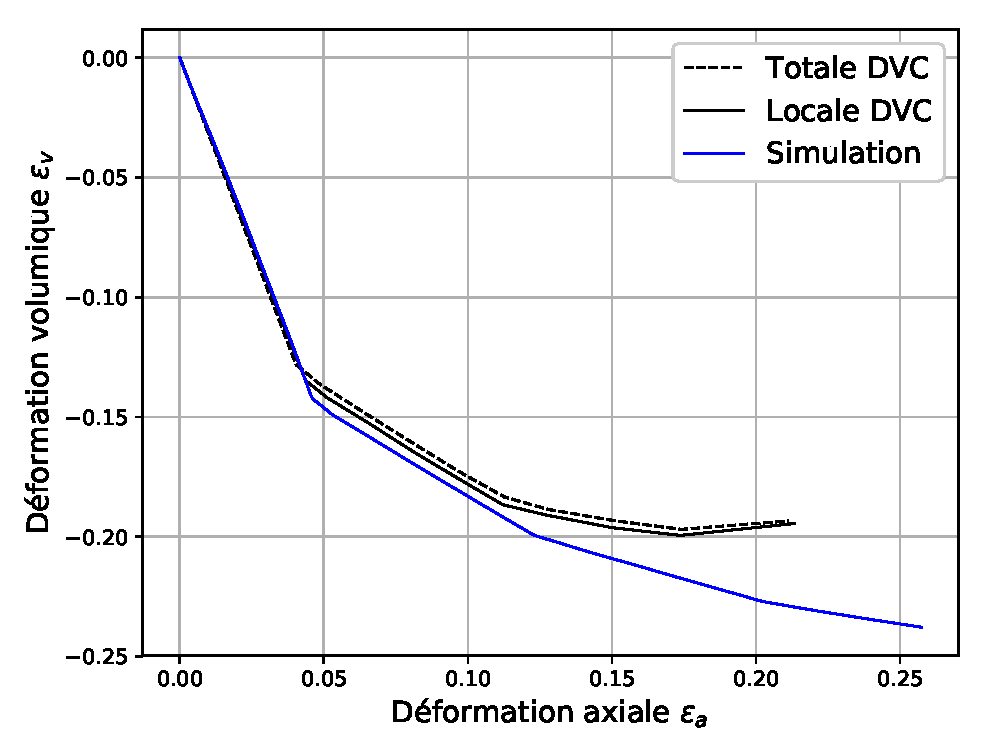
\includegraphics[width=.48\textwidth]{strains_border_size/005_volumique.eps}
				}\\
				\subfloat[Grains pilotés sur une bordure de \SI{135}{\micro\meter}]{
					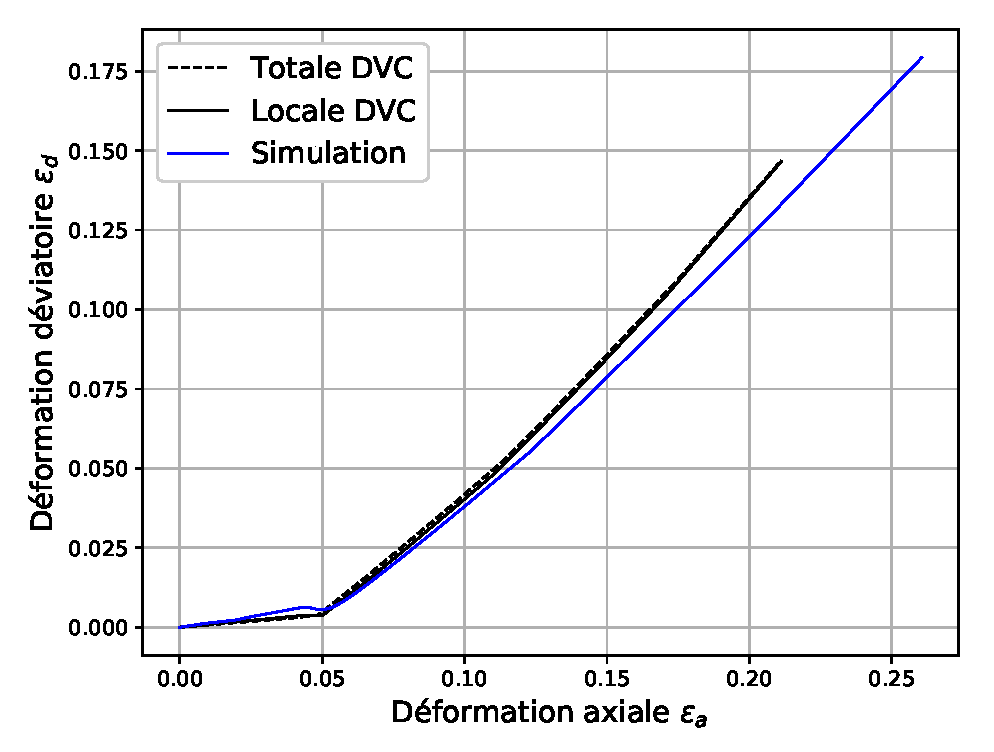
\includegraphics[width=.48\textwidth]{strains_border_size/015_deviatoire.eps}\hfill
					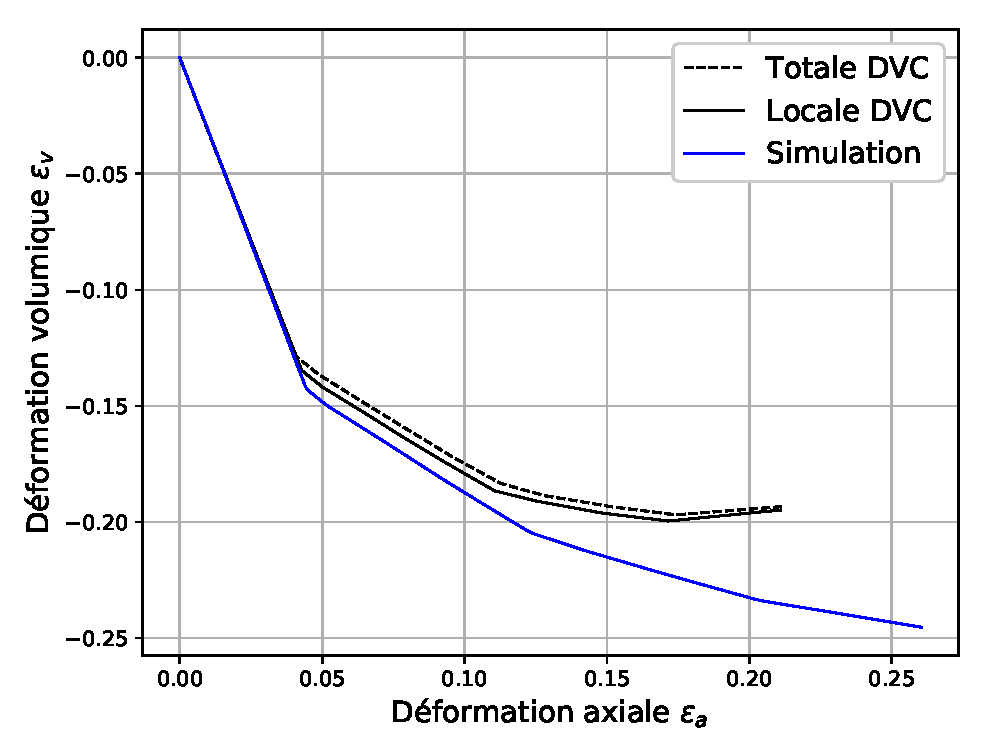
\includegraphics[width=.48\textwidth]{strains_border_size/015_volumique.eps}
				}\\
				\subfloat[Grains pilotés sur une bordure de \SI{225}{\micro\meter}]{
					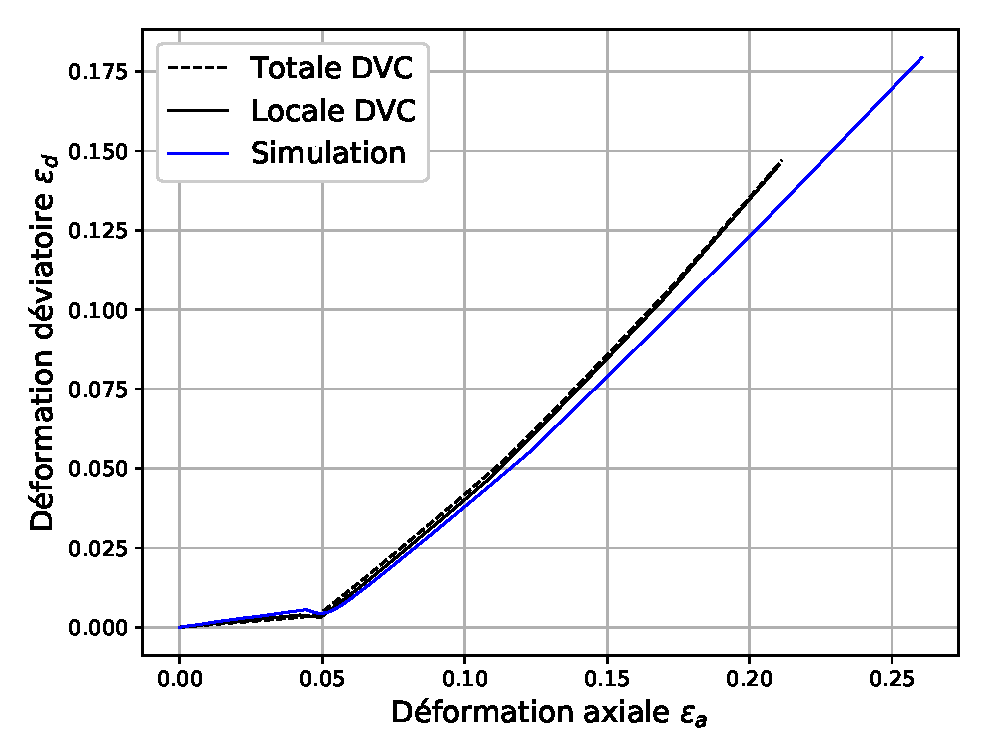
\includegraphics[width=.48\textwidth]{strains_border_size/025_deviatoire.eps}\hfill
					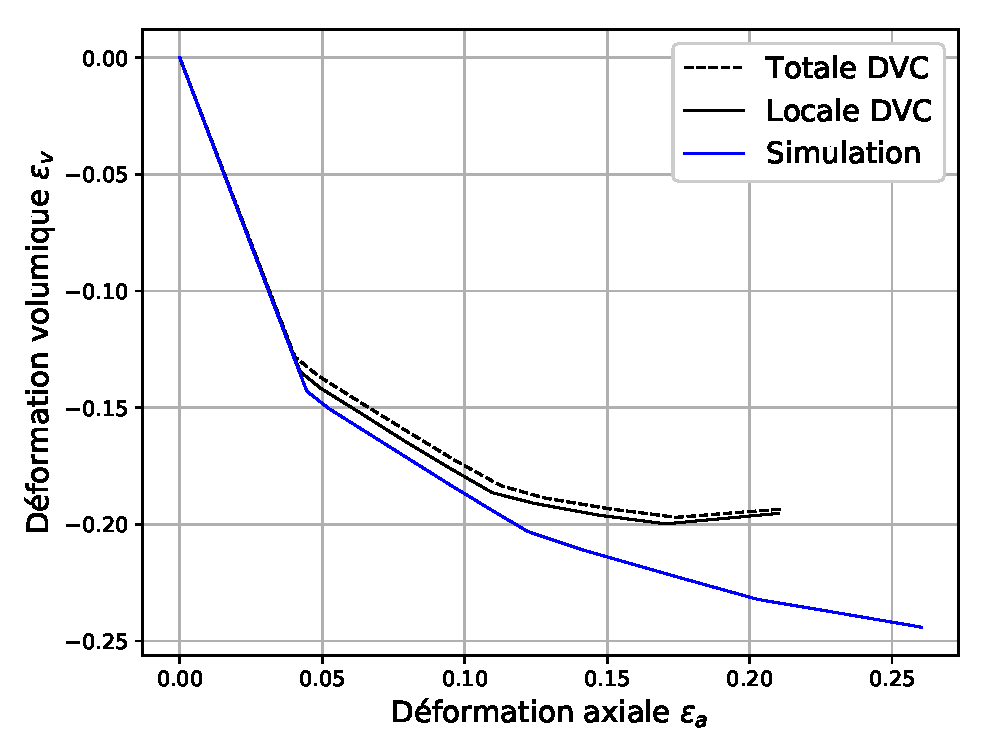
\includegraphics[width=.48\textwidth]{strains_border_size/025_volumique.eps}
				}\\
				\caption{\label{fig06:comparaison_defo_bordure}Déformations déviatoire (gauche) et volumique (droite) en fonction de la déformation axiale pour différentes épaisseurs de la zone de pilotage des grains. La courbe en trait pointillé noir correspond à la déformation moyenne de l'ensemble de l'échantillon mesurée par DVC ; en trait continu noir celle mesurée localement par DVC ; et en trait continu bleu celle mesurée localement dans la simulation.}
			\end{figure}
			\\Il est observé sur la figure \ref{fig06:comparaison_defo_bordure} que l'épaisseur de la zone de pilotage des grains n'affecte pas les conditions aux limites imposées à l'échantillon numérique. En effet, cette figure présente les déformations mésoscopiques calculées par la simulation et par la corrélation pour différentes épaisseurs de la zone de pilotage. La différence entre les deux courbes est faible quelque soit le nombre de grains pilotés en déplacement. Finalement, le pilotage seul de grains qui sont à une faible distance (un tiers d'un grain moyen) de la bordure suffit à observer des conditions aux limites proches de celles observées par la corrélation d'images 3D. Si la taille de la zone de pilotage ne semble pas vraiment jouer un rôle important sur la validité des conditions aux limites, il est a noter qu'elle joue un rôle important dans le calcul des contraintes mésoscopiques dans l'échantillon.
			\begin{figure}\centering
				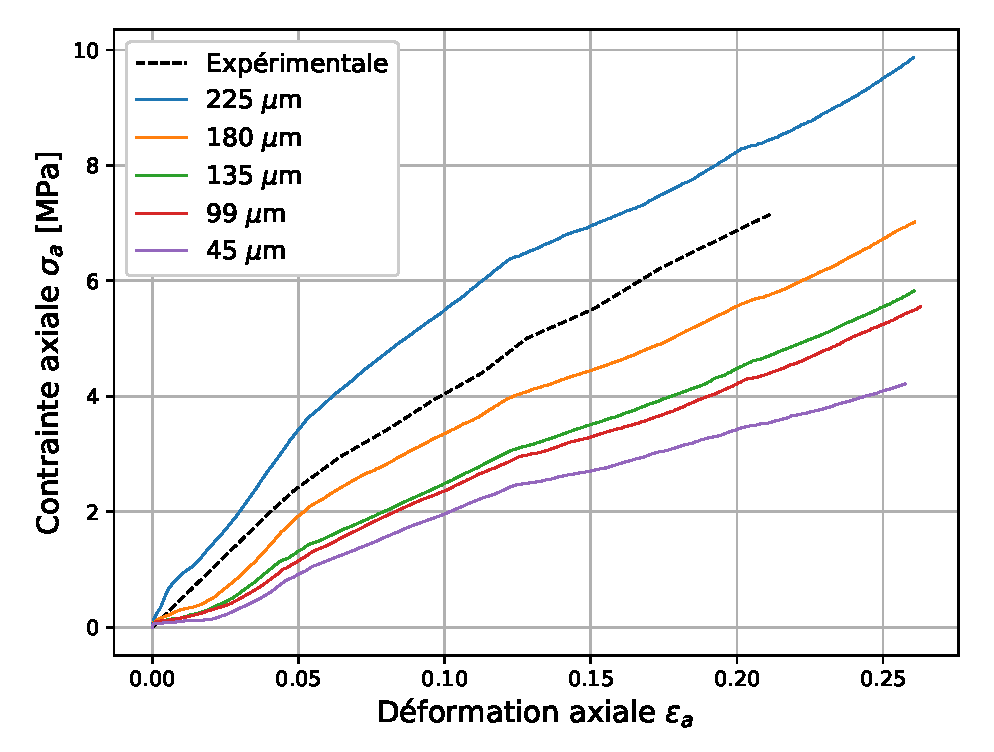
\includegraphics[width=.7\textwidth]{stress_border_size_inside.eps}
				\caption{\label{fig06:contraintes_bordure}Effet de l'épaisseur de la zone de pilotage des grains sur la contrainte moyenne calculée par rapport à la déformation axiale. Le trait en pointillés noirs indique l'évolution de la contrainte axiale mesurée expérimentalement sur l'ensemble de l'échantillon. Ceux en traits continus indique la valeur de la contrainte axiale locale calculée par la simulation pour différentes zones de pilotage.}
			\end{figure}
			\\Comme le montre la figure \ref{fig06:contraintes_bordure}, qui représente l'évolution de la contrainte axiale mésoscopique dans le sous-volume en fonction du chargement axial, la contrainte augmente avec l'épaisseur de la zone de pilotage des grains, quelque soit la déformation axiale imposée. Lorsque le nombre de grains pilotés en déplacement est trop important, le volume numérique devient sur-contraint. Cela est lié au fait que les déplacements imposés aux grains numérisés ne sont pas exactement ceux des grains réels : les déplacements sont choisis par une interpolation linéaire 3D du champ de déplacement obtenu par corrélation mais, surtout, les mouvements de rotation des grains ne sont pas pris en compte et les mouvements de translation sont moyennés sur plusieurs grains dans le pilotage. En plus de cela, la géométrie réelle des grains coupés au niveau de la frontière du sous-volume n'est pas considérée.
			\\Puisque aucune convergence n'est remarquée sur la figure \ref{fig06:contraintes_bordure}, le choix d'une valeur optimale pour l'épaisseur de la zone de pilotage des grains ne peut pas être fait. Des travaux actuels ont pour objectif de rechercher en détail la cause de cet effet. Afin d'éviter de sur-contraindre l'échantillon numérique, l'épaisseur de la zone de pilotage des grains doit être choisie relativement faible puisqu'une telle valeur de l'épaisseur n'affecte pas les conditions aux limites.
	\paragraph{}
	Les études de déformations qui ont été menées jusqu'à présent permettent de valider le fait que les déformations imposées dans les simulations sont très proches de celles réellement observées de manière locale dans les échantillons soumis à la compression triaxiale de révolution dans la limite des états de grandes déformations. Un volume minimal d'approximativement \num{250} grains est nécessaire pour permettre cela (longueur d'arête du sous-volume équivalente à \num{5} à \num{6} grains). Plus la pression de confinement est grande, meilleures sont les simulations aux grandes déformations. Enfin, il est nécessaire de choisir une zone de pilotage des grains suffisamment grande pour considérer le déplacement de tous les grains proches de la frontière du volume mais il est cependant nécessaire de la choisir suffisamment petite pour ne pas sur-contraindre l'échantillon numérique. Une épaisseur de cette zone de \SI{63}{\micro\meter} est choisie pour respecter ces deux conditions.
	\\Puisque les simulations respectent les sollicitations observées localement sur les échantillons réels, il est possible d'étudier le comportement local du milieu granulaire en calculant les états de contraintes et déformations au sein des différents sous-volumes en cours de chargements, et donc en cours de densification. La prochaine partie a pour objectif de présenter l'effet des propriétés mécaniques du matériau sur le comportement moyen du milieu granulaire prédit par simulation.

\section{Caractérisation du matériau constitutif des grains} % Effets matériau sur le comportement méca
	Les simulations qui ont été menées jusqu'à présent permettent d'observer les effets de la méthode numérique qui a été développée sur la cinématique de l'échantillon. Suite à cette analyse des effets numériques et du choix des paramètres optimaux, l'étude de l'influence des paramètres matériau constitutif des grains est envisagée. Pour cela, une zone centrée dans l'échantillon subissant une pression de confinement de \SI{2}{\mega\pascal} est étudiée pour différentes configurations du matériau constitutif des grains. Le sous-volume simulé est cubique et a une longueur d'arête de \SI{900}{\micro\meter} (\num{6} grains de taille moyenne). La zone de pilotage des grains a une épaisseur de \SI{63}{\micro\meter}.
	\\Les propriétés mécaniques du matériau constitutif des grains élasto-plastiques qui sont étudiées sont : le module de Young, la limite d'élasticité, le module d'écrouissage, et enfin, le coefficient de friction statique qui définit les interactions de frottement entre particules.
	\\Le comportement du matériau polystyrène constitutif des grains réels est décrit par un jeu de	paramètres variables inclut dans des intervalles plausibles. En effet, la caractérisation du matériau constitutif des grains réel n’a pas été menée expérimentalement car la taille des grains comme leurs formes complexes rendent cette caractérisation délicate. Il convient également de souligner que les quantités simulées pour cette analyse, par exemple la contrainte axiale simulée, dépendent aussi du réarrangement intergranulaire, de l’augmentation progressive des surfaces de contact entre les grains et d’un niveau d’écrouissage hétérogène et variable dans chaque grain maillé.
	\\Afin d'étudier la réponse mécanique mésoscopique de l'ensemble de grains numérisés avec les propriétés mécaniques imposées, l'analyse des courbes de contrainte en fonction du chargement axial imposé à l'échantillon est faite.
	\paragraph{Module de Young\\}
		\begin{figure}\centering
			\subfloat[Contrainte axiale]{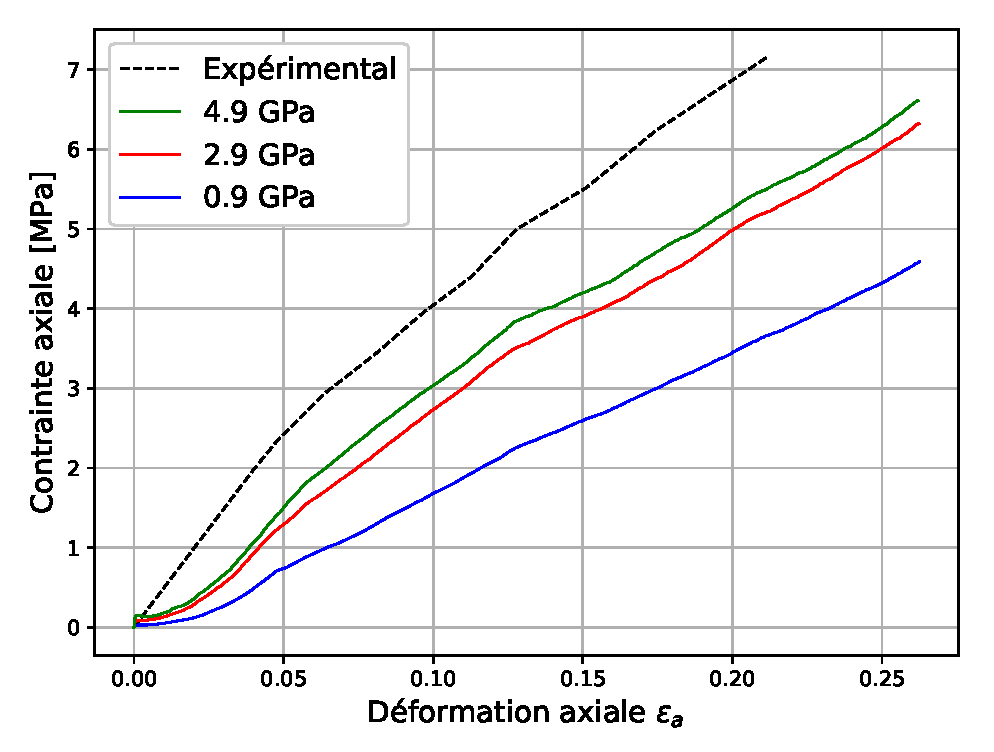
\includegraphics[width=.48\textwidth]{material_effect/E_axial.eps}}\hfill
			\subfloat[Contraintes déviatoire et moyenne]{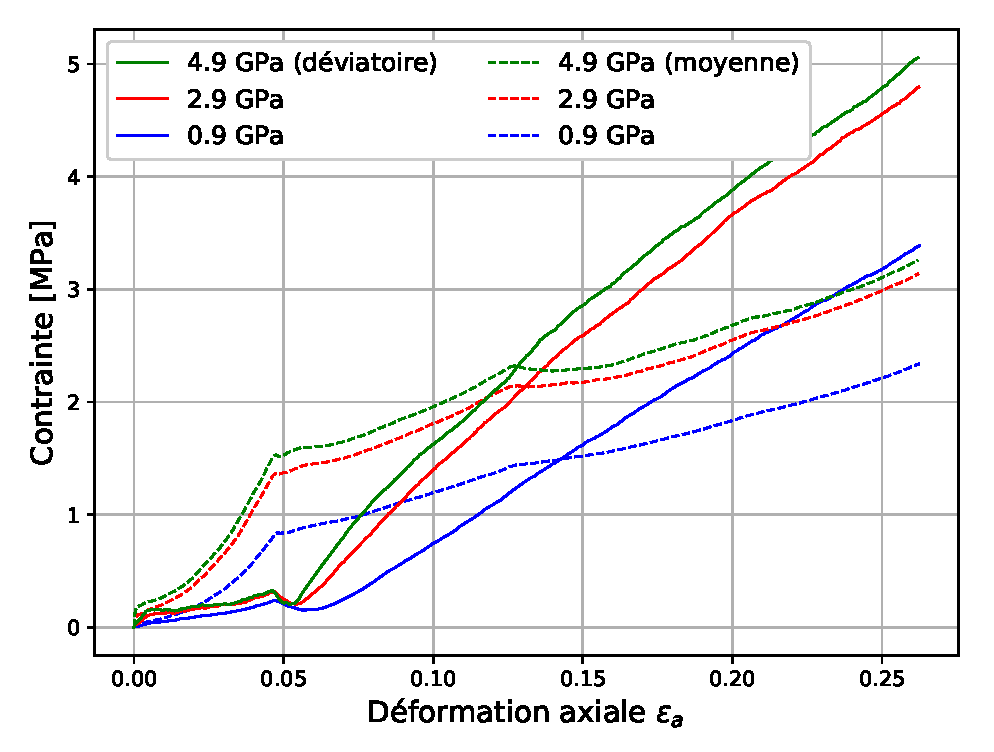
\includegraphics[width=.48\textwidth]{material_effect/E_deviatoire_volumique.eps}}
			\caption{\label{fig06:material_effect_E}Contraintes axiale (a), déviatoire (b - traits pleins) et moyenne (b - traits en pointillés) en fonction de la déformation axiale pour différentes valeurs du module de Young.}
		\end{figure}
		Trois valeurs du module de Young ont été testées : \num{0.9}, \num{2.9} et \SI{4.9}{\giga\pascal}. Pour chacune des simulations présentées ici, la limite élastique du matériau constitutif des grains est de \SI{45}{\mega\pascal}, le module d'écrouissage est de \SI{8.3}{\mega\pascal} et le coefficient de frottement statique est de \num{0.5}. Pour chacune des valeurs du module de Young testées, les courbes de contraintes sont représentées sur la figure \ref{fig06:material_effect_E}. Il est observé que plus le matériau constitutif des grains est rigide, plus la réponse mécanique de l'assemblage de grains est élevée. Un écart du module de Young de \SI{2}{\giga\pascal} (ce qui est plutôt significatif concernant la famille des polymères) pour les deux plus grandes valeurs testées ne présent pas de différence significative en terme de réponse mécanique de l'échantillon. Une augmentation significative de la contrainte apparaît cependant entre les faibles valeurs du module de Young et les valeurs moyennes (relativement à la famille des polymères). Le choix d'un module de Young de \SI{2.9}{\giga\pascal} dans les travaux présentés dans cette thèse, comme indiqué pour le polystyrène dans la littérature \citep{wypych_handbook_2016, matweb}, est cohérent puisque des valeurs inférieures tendent à s'éloigner rapidement du comportement de l'échantillon réellement mesuré (trait en pointillés noirs sur la figure \ref{fig06:material_effect_E}-(a)) et des valeurs plus grandes ne permettent pas de s'en rapprocher significativement.
	\paragraph{Limite élastique\\}
		\begin{figure}\centering
			\subfloat[Contrainte axiale]{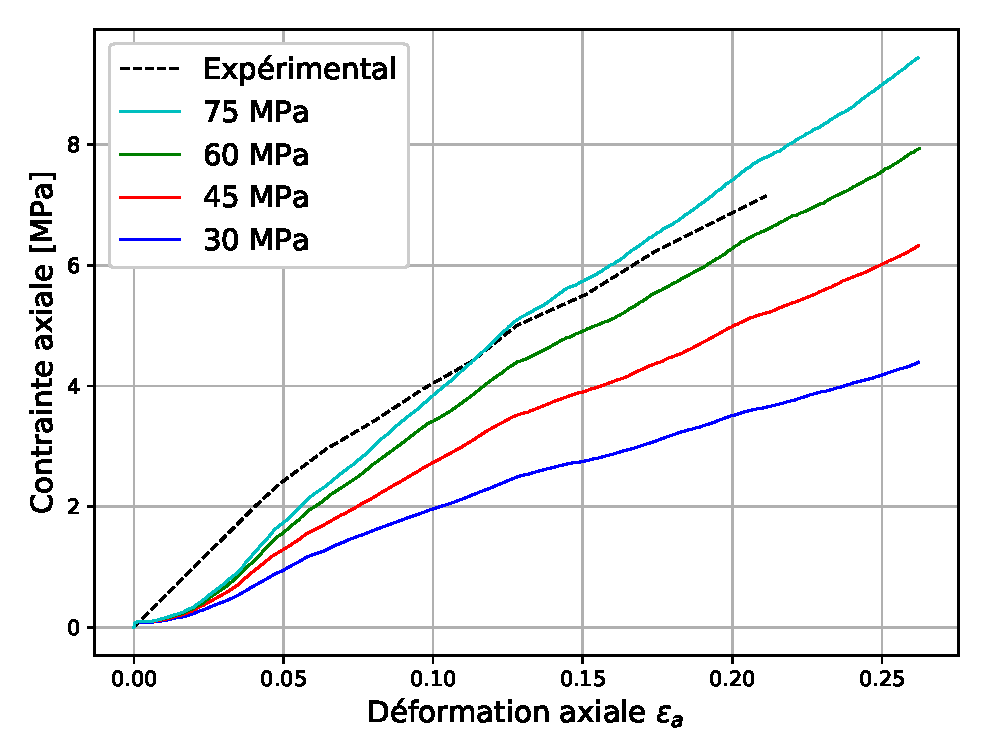
\includegraphics[width=.48\textwidth]{material_effect/Re_axial.eps}}\hfill
			\subfloat[Contraintes déviatoire et moyenne]{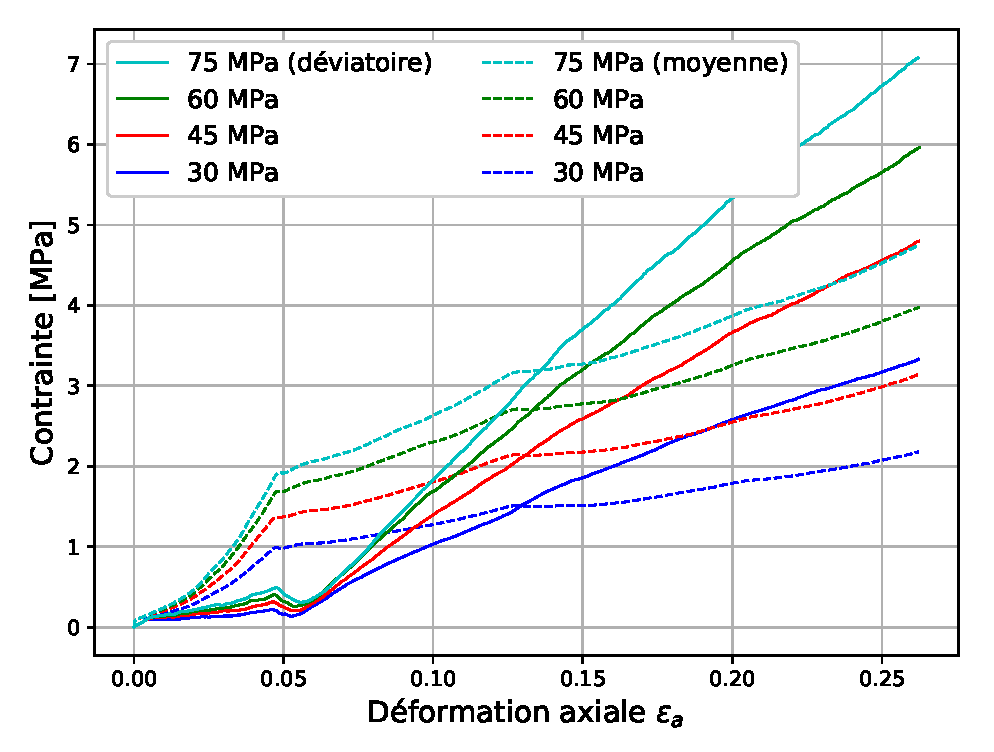
\includegraphics[width=.48\textwidth]{material_effect/Re_deviatoire_volumique.eps}}
			\caption{\label{fig06:material_effect_Re}Contraintes axiale (a), déviatoire (b - traits pleins) et moyenne (b - traits en pointillés) en fonction de la déformation axiale pour différentes valeurs de la limite élastique.}
		\end{figure}
		Avec l'objectif d'étudier l'effet de la limite élastique du matériau constitutif, le module de Young est fixe et prend la valeur de \SI{2.9}{\giga\pascal}. De la même façon que précédemment, le module d'écrouissage est de \SI{8.3}{\mega\pascal} et le coefficient de friction de \num{0.5}. Les valeurs étudiées de la limite élastique sont, quant à elles, de \num{30}, \num{45}, \num{60} et \SI{75}{\mega\pascal}. Les courbes de contraintes pour les différentes valeurs de la limite élastique sont présentées sur la figure \ref{fig06:material_effect_Re}. Il est observé sur ces courbes que la réponse mécanique de l'ensemble de grains est quasi-proportionnelle à la valeur prise par la limite élastique. Les différences de contraintes entre chaque courbe sont relativement grandes et le choix de la limite élastique du matériau est primordiale pour l'étude des contraintes locales. La littérature \citep{wypych_handbook_2016, matweb} indique que la limite élastique du polystyrène est aux alentours de \SI{45}{\mega\pascal} pour des essais de traction. Il est remarqué dans ces travaux qu'une limite élastique plus grande est plus cohérente avec la réponse globale de l'échantillon (trait en pointillés noirs sur la figure \ref{fig06:material_effect_Re}-(a)) en compression. En effet, une valeur de \SI{60}{\mega\pascal} semble plus proche du comportement réel de l'échantillon. Ceci peut s'expliquer par le fait que la limite élastique retenue dans la littérature est une limite en traction simple. Or, en compression et de plus sous confinement, celle-ci pourrait être plus élevée comme le suggère la base de donnée Matweb \citep{matweb}.
	\paragraph{\'Ecrouissage\\}
		\begin{figure}\centering
			\subfloat[Contrainte axiale]{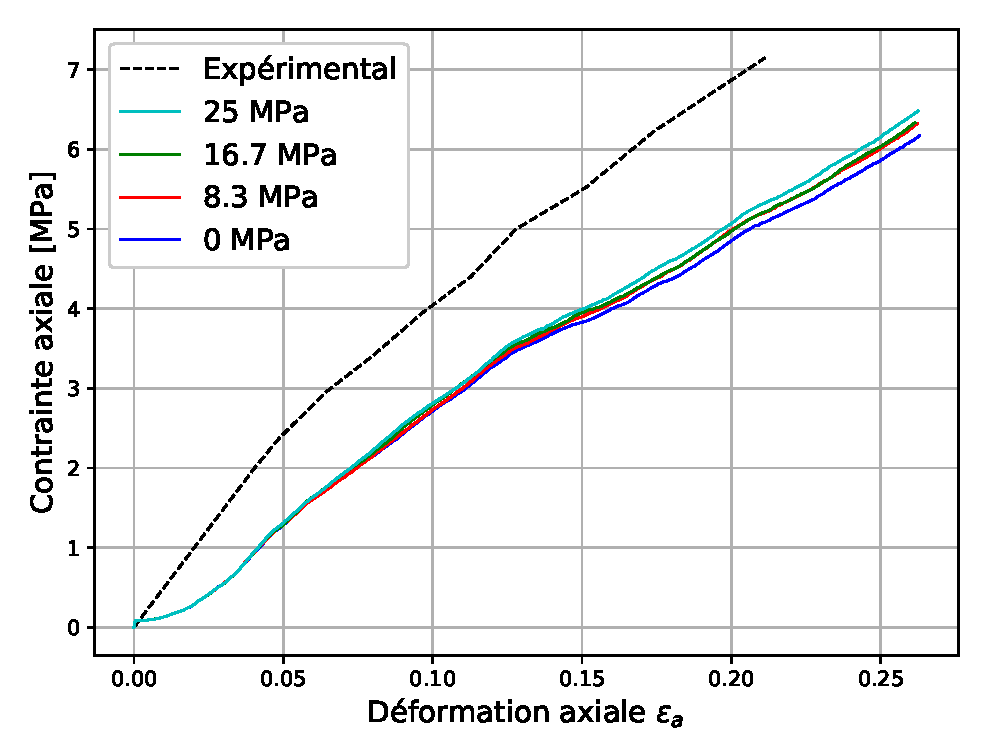
\includegraphics[width=.48\textwidth]{material_effect/Hardening_axial.eps}}\hfill
			\subfloat[Contraintes déviatoire et moyenne]{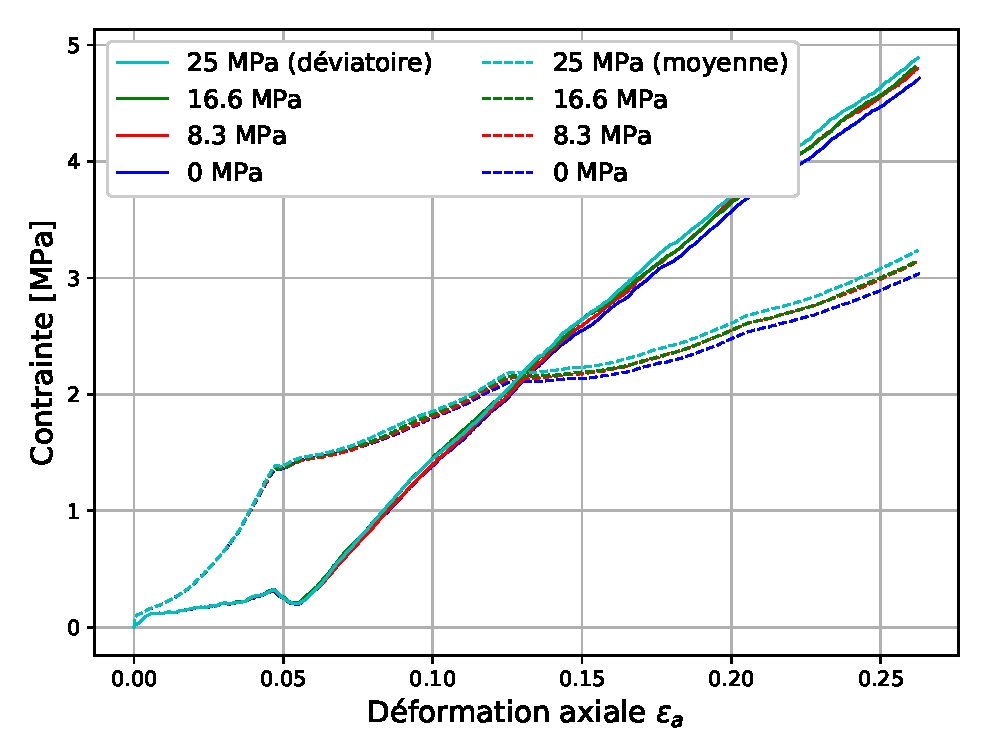
\includegraphics[width=.48\textwidth]{material_effect/Hardening_deviatoire_volumique.eps}}
			\caption{\label{fig06:material_effect_hardening}Contraintes axiale (a), déviatoire (b - traits pleins) et moyenne (b - traits en pointillés) en fonction de la déformation axiale pour différentes valeurs du module d'écrouissage.}
		\end{figure}
		L'effet de l'écrouissage du matériau sur le comportement d'un assemblage de grains est également étudié. Pour analyser ce paramètre matériau dans la simulation, le module de Young est fixé à \SI{2.9}{\giga\pascal}, la limite élastique à \SI{45}{\mega\pascal} et le coefficient de friction à \num{0.5}. Seul le module d'écrouissage varie entre les valeurs de \SI{0}{\mega\pascal} (comportement purement plastique, sans écrouissage), \num{8.3}, \num{16.7} et \SI{25}{\mega\pascal}. Dans ce dernier cas, cela veut dire que pour une déformation plastique de \SI{10}{\percent}, la surface de charge augmente de manière isotrope de \SI{2.5}{\mega\pascal}. La figure \ref{fig06:material_effect_hardening} présente les courbes de contraintes pour ces différentes valeurs du module d'écrouissage. L'analyse des courbes permet d'estimer l'effet de l'écrouissage comme négligeable sur la réponse mécanique de l'ensemble de grains. Bien évidemment, par définition, l'effet de l'écrouissage est plus marqué pour les grandes déformations mais, malgré des modules d'écrouissage relativement différents, la réponse du milieu granulaire est, quant à elle, non significative. Finalement, dans les travaux présentés dans cette thèse, le choix d'un module d'écrouissage pour définir l'importance du durcissement des grains polymériques n'est que peu décisif. Cependant, le choix d'un matériau écrouissable a l'avantage de faciliter la convergence du calcul. Pour cette raison , la valeur de \SI{8.3}{\mega\pascal} a été choisie.
	\paragraph{Frottements aux contacts\\}
		\begin{figure}\centering
			\subfloat[Contrainte axiale]{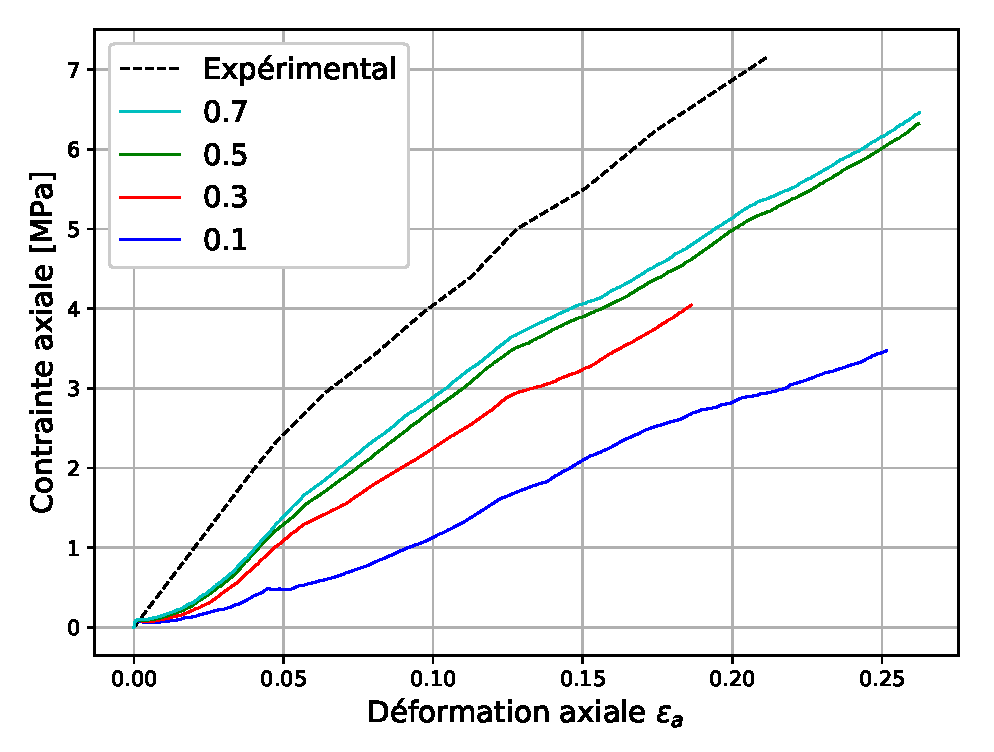
\includegraphics[width=.48\textwidth]{material_effect/Friction_axial.eps}}\hfill
			\subfloat[Contraintes déviatoire et moyenne]{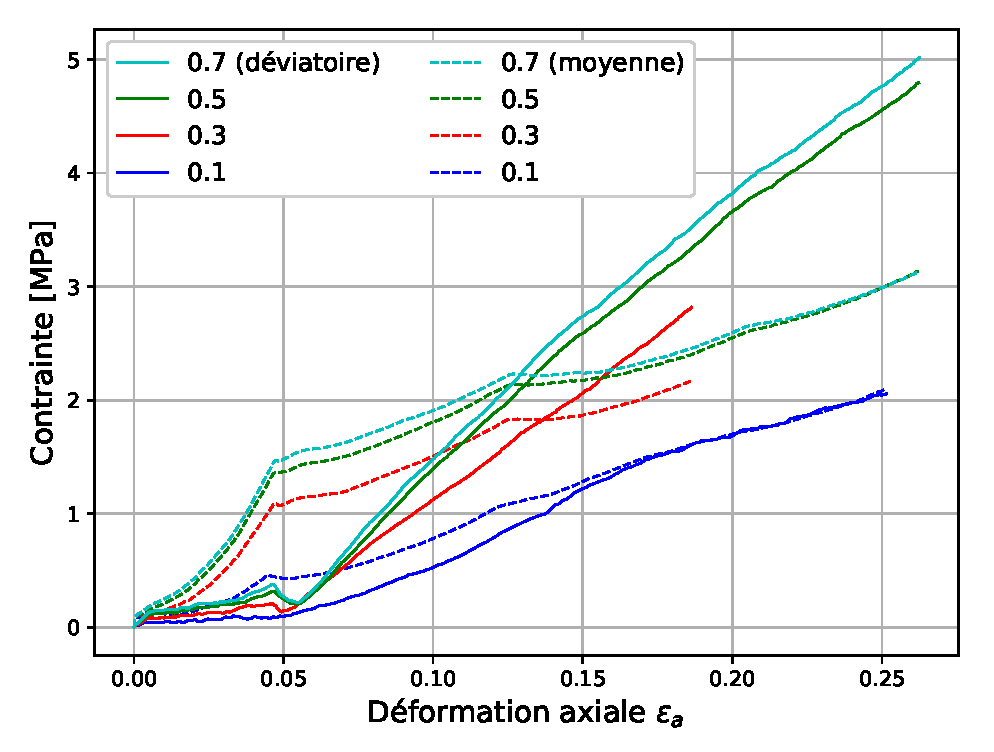
\includegraphics[width=.48\textwidth]{material_effect/Friction_deviatoire_volumique.eps}}
			\caption{\label{fig06:material_effect_friction}Contraintes axiale (a), déviatoire (b - traits pleins) et moyenne (b - traits en pointillés) en fonction de la déformation axiale pour différentes valeurs du coefficient de friction. (La simulation avec le coefficient de friction de \num{0.3} n'a pas été menée jusqu'au dernier état de chargement)}
		\end{figure}
		Le dernier paramètre matériau qui est analysé dans ces travaux est le coefficient de friction statique qui détermine la réponse mécanique de chacun des grains qui sont en contact avec des grains voisins. Dans le but d'étudier cette propriété intrinsèque aux surfaces des grains, plusieurs simulations ont été réalisée avec des coefficients de friction de \num{0.1}, \num{0.3}, \num{0.5} et \num{0.7}. Le module de Young est de \SI{2.9}{\giga\pascal}, la limite élastique est de \SI{45}{\mega\pascal} et le module d'écrouissage de \SI{8.3}{\mega\pascal}. La forme complexe des grains joue un rôle important sur les capacités du milieu granulaire à se réarranger, notamment aux premiers stades de la compression. Pour autant le coefficient de frottement joue également un rôle sur ce même aspect dans un contexte où la pression de confinement est variable suivant les 3 cas étudiés.
		\\La réponse mécanique de l'ensemble de grains pour ces différentes valeurs du coefficient de friction entre grains est présentée sur la figure \ref{fig06:material_effect_friction}. L'observation des ces courbes permet d'observer l'importance du choix de ce paramètre matériau : la contrainte moyenne dans l'échantillon est doublée lorsque le coefficient de friction passe de \num{0.1} à \num{0.5}. Une différence significative de la réponse mécanique du milieu est observée entre les faibles coefficients de friction et les valeurs moyennes. Cependant, la différence est moins significative entre des valeurs relativement élevées du coefficient de frottement. La littérature \citep{wypych_handbook_2016, matweb} indique un coefficient de friction de \num{0.5} pour des contacts polystyrène-polystyrène. Cette valeur est cohérente avec les résultats observés dans ces travaux. En effet, un relativement fort coefficient de friction permet de se rapprocher du comportement mécanique global de l'échantillon (trait en pointillés noirs sur la figure \ref{fig06:material_effect_friction}-(a)). Une valeur plus faible de ce coefficient engendre une baisse significative de la contrainte calculée et un éloignement de la réponse mécanique globale mesurée de l'échantillon. Une valeur plus grande du coefficient n'affecte pas de manière significative la réponse mécanique du milieu.
		
	\paragraph{}
		Les campagnes de simulation qui ont été présentées dans cette partie permettent d'observer l'effet des propriétés mécaniques du matériau constitutif des grains sur le comportement mécanique du milieu granulaire. Il a été observé que le module de Young et le coefficient de friction du matériau ont un effet similaire sur le comportement mécanique du milieu : la réponse mécanique est d'autant plus grande que la valeur de ces propriétés est grande. Ce résultat est significatif entre les faibles valeurs et les valeurs moyennes de ces propriétés mais la différence est peu marquée entre les valeurs moyennes et fortes. L'effet de la limite élastique a également été étudié et il a été observé une proportionnalité approximative entre la réponse mécanique du milieu et la valeur de la limite élastique. Enfin, il a été noté que l'effet de l'écrouissage du matériau est négligeable et n'intervient que dans une très faible mesure pour les grandes déformations.
		\\La comparaison des courbes de contrainte axiale issues de la simulation avec celle de la réponse globale de l'échantillon (mesurée lors de la compression triaxiale) permet d'estimer les propriétés mécaniques du polystyrène. Ainsi, la littérature \citep{wypych_handbook_2016, matweb} indique des valeurs du module de Young et du coefficient de friction, respectivement, de \SI{2.9}{\giga\pascal} et de \num{0.5}. L'utilisation de ces valeurs dans les simulations est cohérente. Cependant, il a été observé qu'une limite élastique en compression de \SI{60}{\mega\pascal} est plus appropriée que celle indiquée dans la littérature pour des essais de tractions (\SI{45}{\mega\pascal}).
		\\Malgré les choix de ces paramètres matériau, la différence entre le comportement global de l'échantillon et le comportement local calculé par les simulations n'est pas négligeable. Le choix de l'épaisseur de la zone de pilotage des grains est un paramètre à prendre en compte pour analyser localement les contraintes et se rapprocher du comportement mécanique global. Comme le montre la figure \ref{fig06:contraintes_bordure}, la contrainte moyenne calculée localement est dépendante de la zone de pilotage. Comme il a été vu dans les paragraphes précédents, il existe une incertitude quand à l'épaisseur de la zone de pilotage des grains qui affecte très significativement la valeur des contraintes.

\section{\'Etude des contraintes mésoscopiques par zones} % Analyse en fonction de l'emplacement dans l'échantillon et de la pression de confinement
	L'analyse des contraintes dans les échantillons soumis à la compression triaxiale est menée par l'intermédiaire de simulations numériques de sous-volumes localisés à différentes positions dans les échantillons. Le matériau constitutif des grains pour l'étude des contraintes possède un module de Young de \SI{2.9}{\giga\pascal}, une limite élastique de \SI{45}{\mega\pascal} et un coefficient de friction de \num{0.5}. Les volumes simulés sont cubiques est ont une longueur d'arête de \SI{900}{\micro\meter} (\num{6} grains de taille moyenne). La zone de pilotage des grains à une épaisseur de \SI{63}{\micro\meter}. L'évolution de la contrainte moyenne est calculée pour des sous-volumes situés sur la hauteur médiane du volume de tomographie et pour des positions radiales centrées et excentrées.
	\begin{figure}\centering
		\begin{minipage}[c]{0.49\textwidth}\centering
			\tdplotsetmaincoords{80}{120}
			\begin{tikzpicture}[scale=.6, tdplot_main_coords]
				% dessine les axes
				\begin{scope}[shift={(0,-6.5,0)}]
					\draw[->] (0,0,0) -- ++(2,0,0) node[below]{$x$};
					\draw[->] (0,0,0) -- ++(0,1.5,0) node[below]{$y$};
					\draw[->] (0,0,0) -- ++(0,0,1.5) node[left]{$z$};
				\end{scope}
				% dessine le cylindre
				\pgfmathsetmacro{\angleOffset}{30}
				\draw[dashed] (0,0,0) ++ (90+\angleOffset:3) arc (90+\angleOffset:270+\angleOffset:3);
				\draw[] (0,0,0) ++ (-90+\angleOffset:3) arc (-90+\angleOffset:90+\angleOffset:3);
				\draw[] (0,0,10) circle (3);
				\draw[] (0,0,10) ++ (-90+\angleOffset:3) -- ++(0,0,-10);
				\draw[] (0,0,10) ++ (90+\angleOffset:3) -- ++(0,0,-10);
				% dessine l'axe du cylindre
				\draw[blue, dash dot dot] (0,0,-1) -- (0,0,11);
				\filldraw[blue, opacity=.3] (0,0,0) circle (0.2);
				\filldraw[blue, opacity=.8] (0,0,10) circle (0.2);
				% dessine l'axe selon x
				\draw[red, dash dot dot] (-4,0,5) -- (4,0,5);
				\tdplotsetthetaplanecoords{90}
				\filldraw[red, opacity=.3, tdplot_rotated_coords] (5,0,3) circle (0.15);
				\filldraw[red, opacity=.8, tdplot_rotated_coords] (5,0,-3) circle (0.15);
				% dessine l'axe selon y
				\draw[orange, dash dot dot] (0,-4,5) -- (0,4,5);
				\tdplotsetthetaplanecoords{0}
				\filldraw[orange, opacity=.3, tdplot_rotated_coords] (5,0,-3) circle (0.2);
				\filldraw[orange, opacity=.8, tdplot_rotated_coords] (5,0,3) circle (0.2);
				% dessine les sous volumes
				\newcommand{\makeCube}[5]{
					\fill[#5, opacity=0.5] (#1-#4/2.,#2-#4/2.,#3-#4/2) -- ++(0,#4,0) -- ++(0,0,#4) -- ++(0,-#4,0) -- cycle;
					\fill[#5, opacity=0.5] (#1-#4/2.,#2-#4/2.,#3-#4/2) -- ++(#4,0,0) -- ++(0,0,#4) -- ++(-#4,0,0) -- cycle;
					\fill[#5, opacity=0.5] (#1-#4/2.,#2-#4/2.,#3-#4/2) -- ++(0,#4,0) -- ++(#4,0,0) -- ++(0,-#4,0) -- cycle;
					\fill[#5, opacity=0.5] (#1-#4/2.,#2+#4/2.,#3-#4/2) -- ++(#4,0,0) -- ++(0,0,#4) -- ++(-#4,0,0) -- cycle;
					\fill[#5, opacity=0.5] (#1-#4/2.,#2-#4/2.,#3+#4/2) -- ++(#4,0,0) -- ++(0,#4,0) -- ++(-#4,0,0) -- cycle;
					\draw[#5] (#1+#4/2.,#2-#4/2.,#3-#4/2) -- ++(0,#4,0) -- ++(0,0,#4) -- ++(0,-#4,0) -- cycle;
					\draw[#5] (#1+#4/2.,#2+#4/2.,#3-#4/2) -- ++(-#4,0,0) -- ++(0,0,#4) -- ++(#4,0,0) -- cycle;
					\draw[#5] (#1+#4/2.,#2-#4/2.,#3+#4/2) -- ++(-#4,0,0) -- ++(0,#4,0);
				}
				\pgfmathsetmacro{\sizeA}{.5}
				\pgfmathsetmacro{\radialDist}{2}
				% dessine la distance radiale
				\draw[dotted] (0,0,5) circle (\radialDist);
				\makeCube{0}{0}{4.5}{\sizeA}{blue}
				\makeCube{0}{0}{5}{\sizeA}{blue}
				\makeCube{0}{0}{5.5}{\sizeA}{blue}
				\makeCube{-\radialDist}{0}{5}{\sizeA}{red}
				\makeCube{0}{-\radialDist}{5}{\sizeA}{orange}
				\makeCube{\radialDist}{0}{5}{\sizeA}{red}
				\makeCube{0}{\radialDist}{5}{\sizeA}{orange}
			\end{tikzpicture}
		\end{minipage}
		\begin{minipage}[c]{.5\textwidth}\centering
			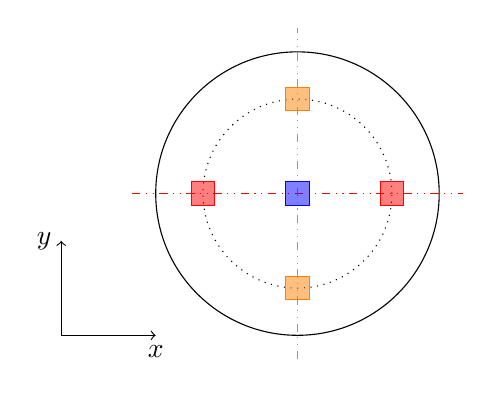
\begin{tikzpicture}[scale=.6]
				\pgfmathsetmacro{\sizeA}{.5}
				\pgfmathsetmacro{\radialDist}{2}
				% dessine le repère
				\begin{scope}[shift={(-2,0)}]
					\draw[->] (0,0) -- ++(2,0) node[below]{$x$};
					\draw[->] (0,0) -- ++(0,2) node[left]{$y$};
				\end{scope}
				% dessine l'échantillon
				\draw[] (3,3) circle (3);
				% dessine les axes
				\draw[red, dash dot dot] (-.5,3) -- ++(7,0);
				\draw[orange, dash dot dot] (3,-.5) -- ++(0,7);
				% dessine la distance radiale
				\draw[dotted] (3,3) circle (\radialDist);
				% dessine les sous-volumes
				\filldraw[blue, fill opacity=.5] (3-\sizeA/2,3-\sizeA/2) rectangle ++(\sizeA,\sizeA);
				\filldraw[red, fill opacity=.5] (3-\radialDist-\sizeA/2,3-\sizeA/2) rectangle ++(\sizeA,\sizeA);
				\filldraw[red, fill opacity=.5] (3+\radialDist-\sizeA/2,3-\sizeA/2) rectangle ++(\sizeA,\sizeA);
				\filldraw[orange, fill opacity=.5] (3-\sizeA/2,3-\radialDist-\sizeA/2) rectangle ++(\sizeA,\sizeA);
				\filldraw[orange, fill opacity=.5] (3-\sizeA/2,3+\radialDist-\sizeA/2) rectangle ++(\sizeA,\sizeA);
			\end{tikzpicture}
		\end{minipage}
		\caption{\label{fig06:stress_sample_location}Placement des volumes simulés (cubes colorés) par rapport à l'échantillon réellement testé (cylindre en trait noir). L'étude des contraintes est réalisée au centre de l'échantillon (cubes bleus) et sur quatre positions excentrées sur la hauteur médiane (cubes rouges et oranges).}
	\end{figure}
	La figure \ref{fig06:stress_sample_location} donne une illustration du positionnement des sous-volumes simulés par rapport à un des échantillons cylindrique soumis à la compression. Cette étude a été menée sur chacun des trois échantillons dont les pressions de confinement sont de \num{1}, \num{2} et \SI{7}{\mega\pascal}. Les contraintes dans la zone centrale des échantillons sont moyennées sur trois simulations centrées radialement et autour de la hauteur médiane de l'échantillon (les trois cubes bleus représentés sur la figure \ref{fig06:stress_sample_location}). Les contraintes excentrées sont moyennées, quant à elles, sur quatre simulations dans la hauteur médiane de l'échantillon et à une distance radiale de \SI{2.7}{\milli\meter} de l'axe médian de l'échantillon (les cubes rouges et oranges sur la figure \ref{fig06:stress_sample_location}).
	\begin{figure}\centering
		\subfloat[Pression de confinement : \SI{1}{\mega\pascal}]{
			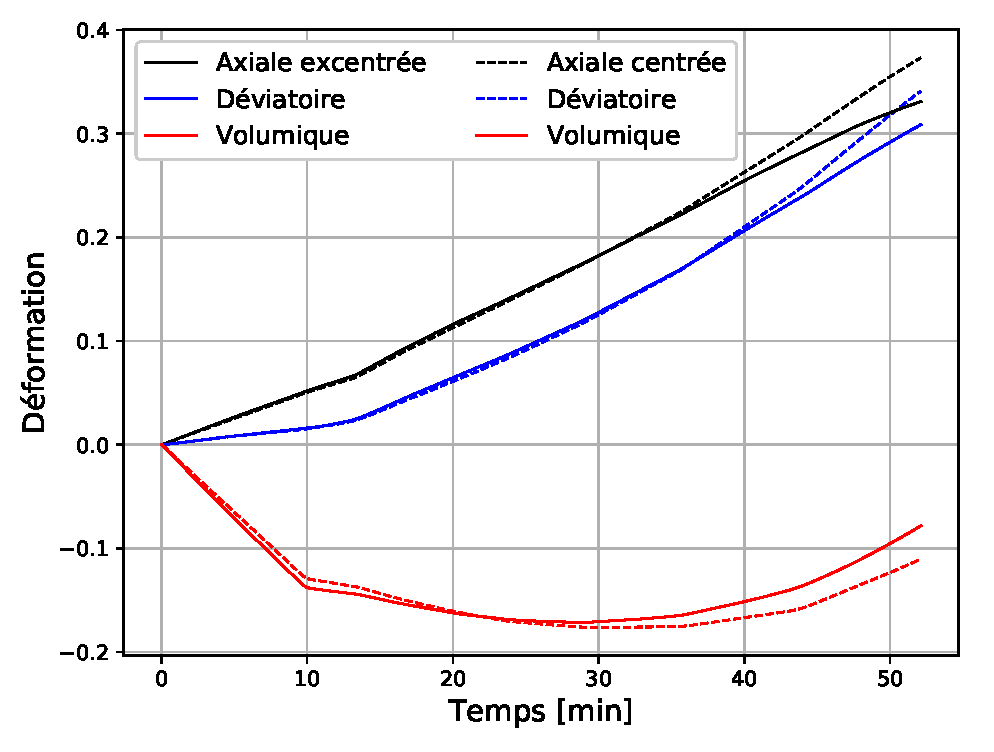
\includegraphics[width=.49\textwidth]{locations/1_MPa_strains.eps}\hfill
			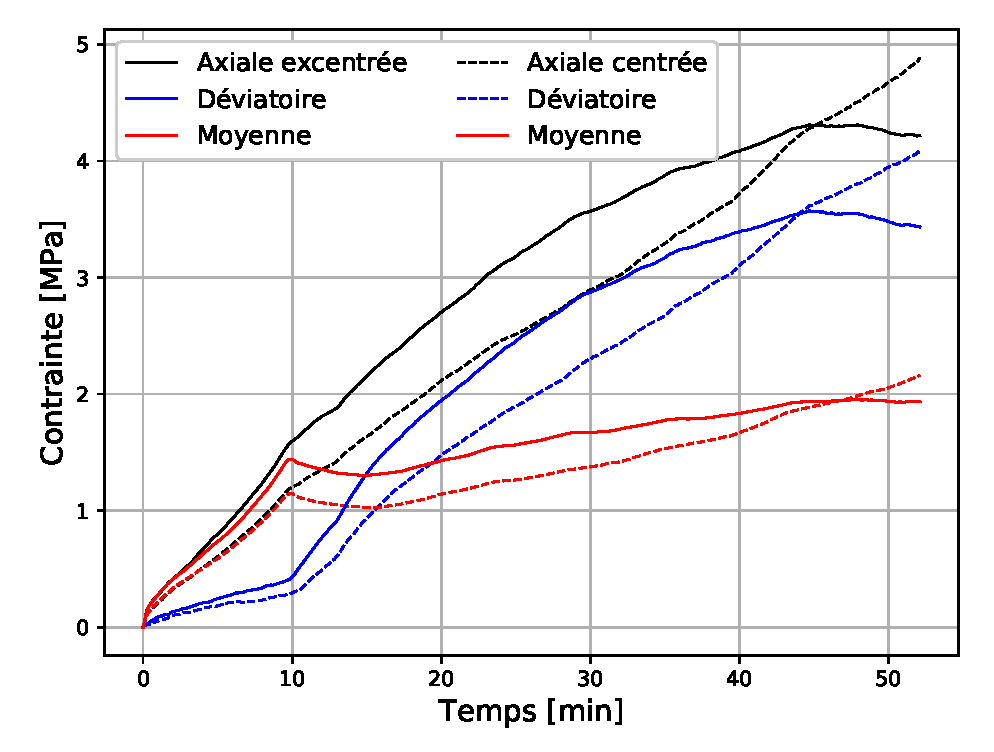
\includegraphics[width=.49\textwidth]{locations/1_MPa_stresses.eps}
		}\\
		\subfloat[Pression de confinement : \SI{2}{\mega\pascal}]{
			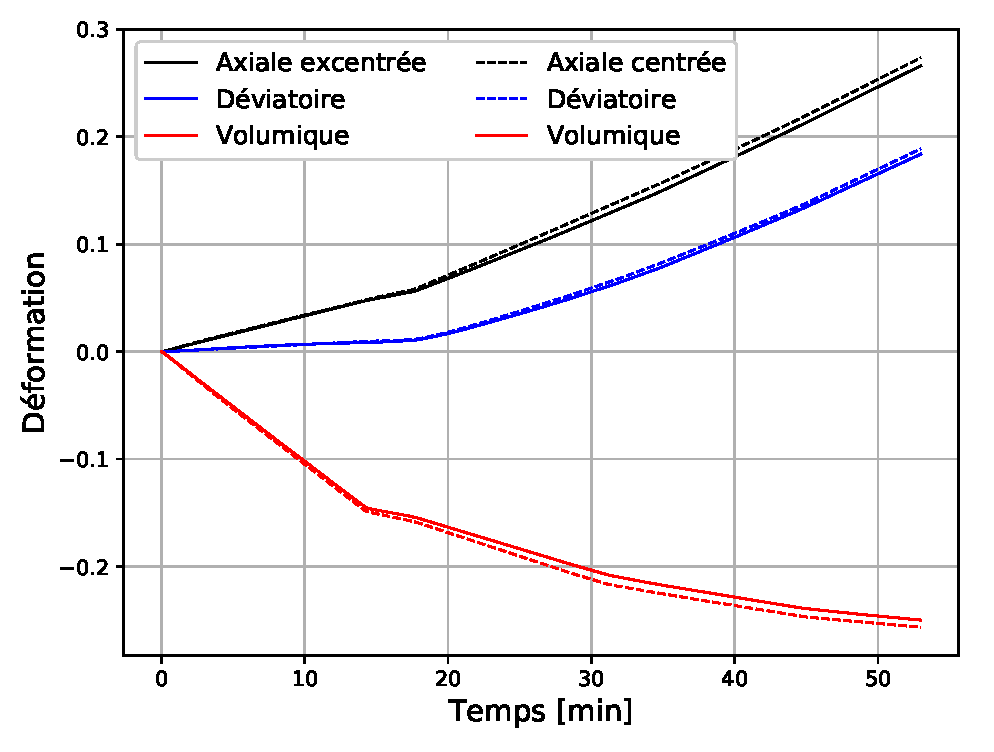
\includegraphics[width=.49\textwidth]{locations/2_MPa_strains.eps}\hfill
			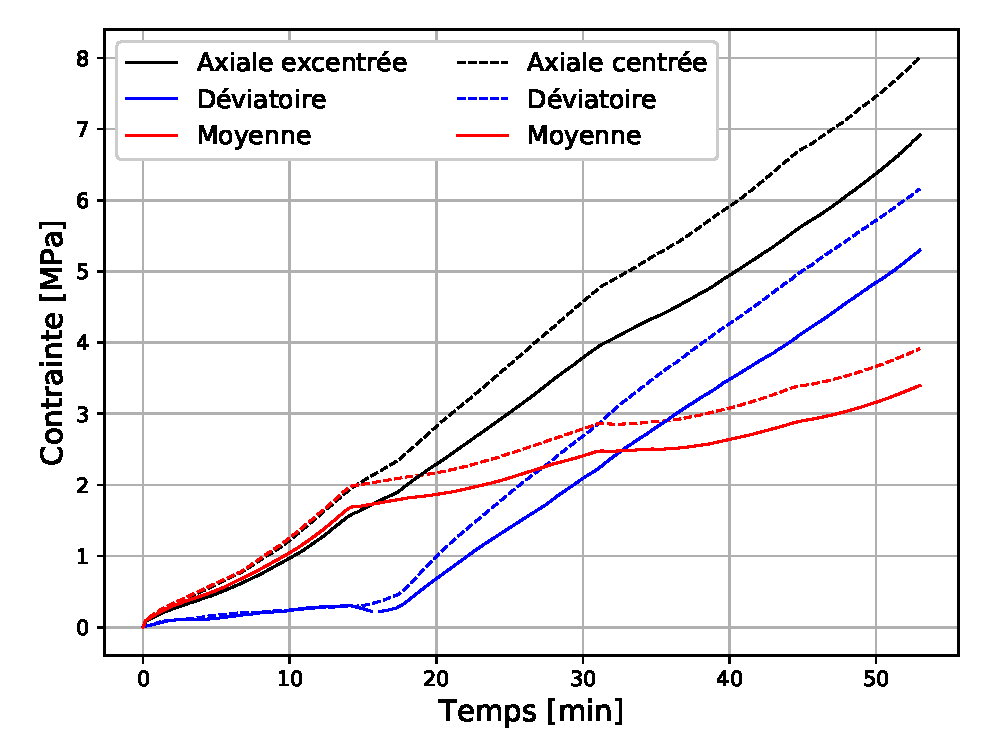
\includegraphics[width=.49\textwidth]{locations/2_MPa_stresses.eps}
		}\\
		\subfloat[Pression de confinement : \SI{7}{\mega\pascal}]{
			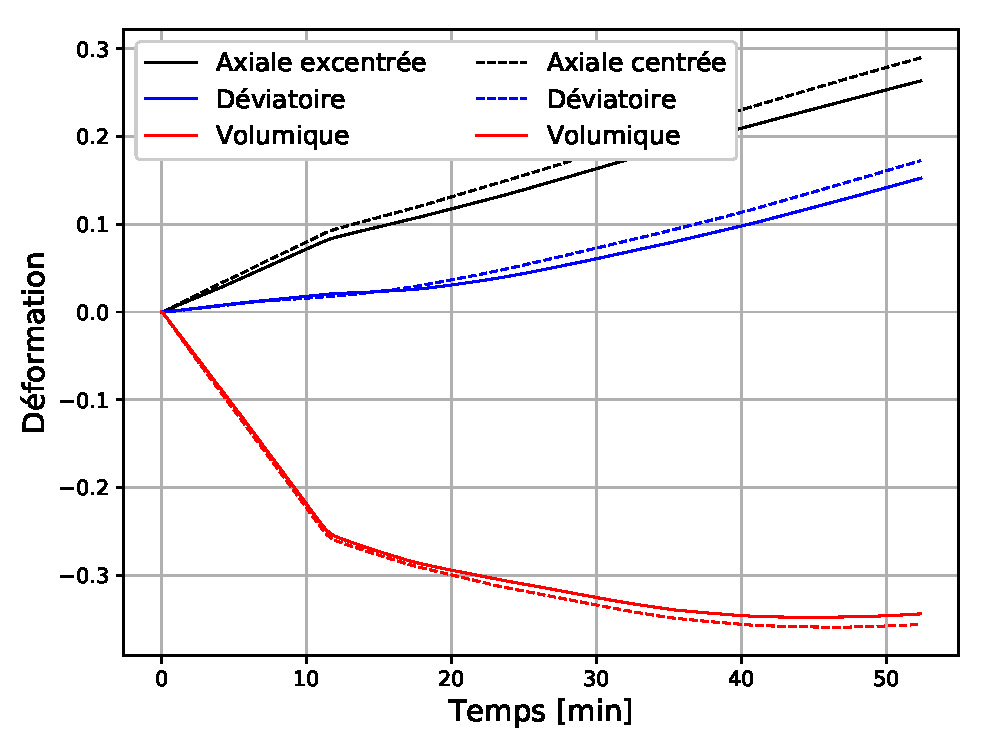
\includegraphics[width=.49\textwidth]{locations/7_MPa_strains.eps}\hfill
			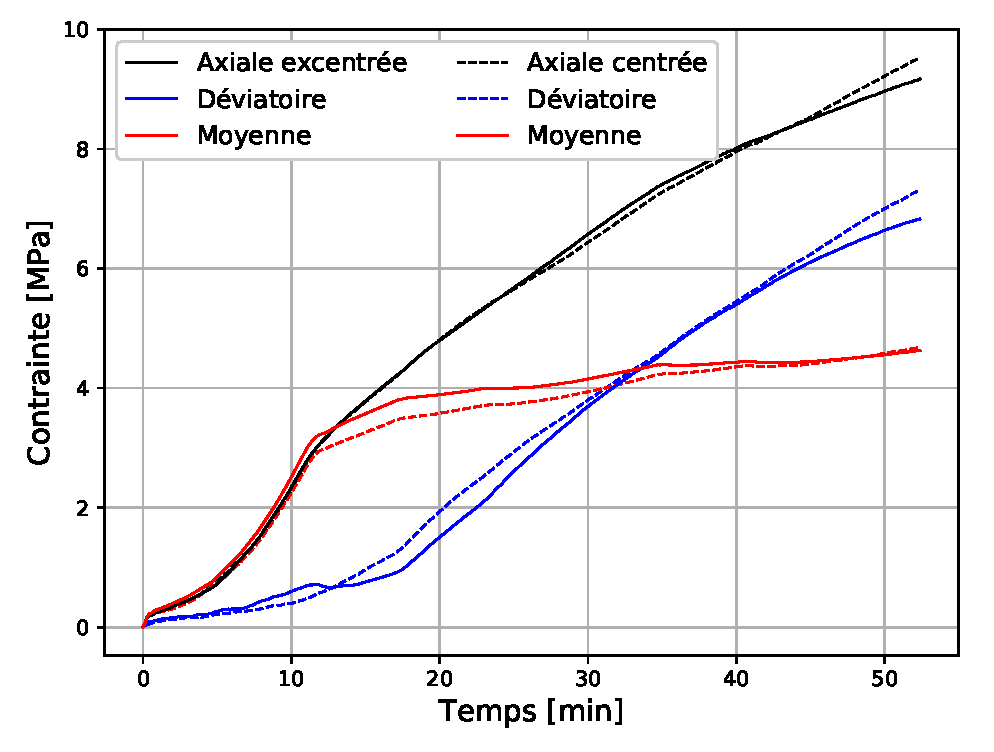
\includegraphics[width=.49\textwidth]{locations/7_MPa_stresses.eps}
		}
		\caption{\label{fig06:contraintes_radial}Courbes des déformations (à gauche) et contraintes (à droite) axiales (traits noirs), déviatoires (traits bleus) et volumiques / moyenne (traits rouges) en fonction du temps de chargement pour les sous-volumes centrés radialement (traits en pointillés) et les sous-volumes excentrés (traits continus) et pour chacun des échantillons.}
	\end{figure}
	\\La figure \ref{fig06:contraintes_radial} présente l'ensemble des courbes de contraintes et déformations pour les zones centrées (traits en pointillés) et excentrées (traits continus). Afin de permettre la comparaison des courbes, il a été choisi de les représenter en fonction du temps de chargement. La durée de chargement considérée (de l'ordre de l'heure) n'est pas celle de l'expérimentation (\num{2} jours), il s'agit en fait de la durée réelle de chargement - c'est à dire lorsque le piston est en mouvement avec une vitesse constante de \SI[per-mode=symbol]{2}{\micro\meter\per\second}.
	\\Les courbes présentées montrent que pour la pression de confinement de \SI{7}{\mega\pascal}, les contraintes sont relativement homogènes dans la zone explorée de l'échantillon. En revanche, pour les pressions de confinement de \num{1} et \SI{2}{\mega\pascal} on constate une différence entre les contraintes calculées au centre de l'échantillon et à une distance de 2.7mm de l'axe médian. Ce comportement est très probablement dû au frottement entre les grains qui, en s'opposant au mouvement relatif des particules et à la transmission des contraintes (par le biais de mécanismes de type 'effet d'arche' mentionnés au chapitre \ref{chap:biblio}), génère des gradients de contrainte et de déformation au sein de l'échantillon. La pression de confinement de \SI{7}{\mega\pascal} semble suffisante pour dépasser la résistance du frottement, probablement en mobilisant la déformation des grains.
	\\Il est observé de plus que pour la pression de confinement de \SI{1}{\mega\pascal}, les trois composantes de contrainte sont systématiquement plus élevées que les contraintes dans la zone excentrée (jusqu'à environ \SI{45}{\minute}). À l'inverse, pour la pression de confinement de \SI{2}{\mega\pascal}, la contrainte est plus élevée au centre.
	\\Il est difficile d'estimer la variabilité spatiale des contraintes calculées par la simulation en fonction des particularités des sous-volumes choisis. Comme précisé plus haut, les contraintes ont été moyennées sur plusieurs sous-volumes afin de limiter cette variabilité, mais il se peut qu'elle ait une influence non nulle sur les résultats observés.
	\\Néanmoins, si la tendance observée sur les courbes est avérée, la différence de comportement entre les pressions de confinement de \num{1} et \SI{2}{\mega\pascal} suggère une mécanisme de transmission des contraintes différent. Pour la pression de \SI{1}{\mega\pascal}, la zone centrale de l'échantillon voit, relativement à la zone excentrée, des contraintes plus faibles pour des déformations presque identiques, ce qui pourrait correspondre au comportement d'un milieu ayant une densité plus faible. Effectivement, on peut constater que la déformation volumique est légèrement plus faible pour la zone centrale de l'échantillon. Pour la pression de confinement de \SI{2}{\mega\pascal}, au contraire la contrainte (toutes composantes confondues) est plus importante au centre que dans la zone excentrée. Il est observé de plus que cette fois, la zone centrale et la zone excentrée voient une déformation volumique approximativement égale (voire très légèrement supérieure pour la zone centrale). La pression de \SI{2}{\mega\pascal} est apparemment suffisante pour contrebalancer les forces de frottement entre grains et densifier l'échantillon à c\oe{}ur. Par suite, la partie centrale de l'échantillon supporte le chargement (et ce d'autant plus que la déformation axiale augmente), tandis que les zones périphériques, plus libres, sont moins sollicitées.
	\\Deux remarques supplémentaires peuvent être faites sur les résultats de l'essai à la pression de confinement de \SI{1}{\mega\pascal}.
	L'apparition de la dilatance pour un temps de l'ordre de 30 minutes (la courbe de déformation volumique change de pente) est constatée. En même temps, une modification du comportement mécanique des sous-volumes simulés est observée : la différence entre la zone centrale et la zone excentrée augmente tant pour les déformations que pour les contraintes. Dans la zone excentrée, les déformations axiale et déviatoire augmentent moins vite et les contraintes augmentent moins vite et finissent même par diminuer. En effet les résultats de corrélation de volumes montrent qu'une bande de cisaillement caractérisée par une localisation de la contrainte déviatoire commence à apparaître en fin d'essai, en particulier dans la partie centrale (cf. figure \ref{fig04:champs_deformations} du chapitre \ref{chap:experimental}).
	La deuxième remarque se rapporte à la diminution de la pente de la courbe de contrainte moyenne immédiatement après l'étape de confinement. Cet effet, non visible sur les résultats des essais à pression de confinement supérieure, est très probablement un effet de la surconsolidation à \SI{2}{\mega\pascal}. Il est à noter que cette surconsolidation n'est pas directement visible sur les courbes de contrainte pour la raison que lors de l'essai, le scan est effectué après décharge à la pression de confinement de \SI{1}{\mega\pascal}. Les déplacements lors du confinement à \SI{2}{\mega\pascal} n'ont donc pas été mesurés par corrélation d'image et la simulation numérique impose aux grains des déplacements menant directement à l'état déchargé sans passer par le confinement à \SI{2}{\mega\pascal}. Ainsi la contrainte calculée est intermédiaire. Il peut être supposé que cette surconsolidation participe à amplifier le phénomène de dilatance, comme il a été observé pour les poudres ductiles, quoique dans des conditions de confinement bien plus sévères \citep{pavier_caracterisation_1998}.
	
\paragraph{}
	Les résultats présentés dans cette dernière partie illustre la manière d'analyser le champ de contrainte mésoscopique dans l'échantillon grâce aux simulations menées en différentes zones dans l'échantillon. Cela est rendu possible car les simulations sont menées avec des conditions aux limites proches de celles réellement observées dans les échantillons issus des essais expérimentaux. La comparaison et l'analyse des déformations locales calculées par corrélation de volumes et par simulation a permis de valider la méthode numérique.
	\\Bien que la méthode numérique soit correcte, les propriétés mécaniques du matériau constitutif des grains dans les simulations doivent être définies correctement pour simuler de la manière la plus réelle possible le comportement mécanique du milieu granulaire. Pour le polystyrène (PS) avec une loi de comportement élasto-plastique, il a été vu que l'effet de l'écrouissage sur le comportement du milieu est négligeable contrairement au module de Young, du coefficient de frottement et de la limite élastique. Il a été vu qu'un module de Young de \SI{2.9}{\giga\pascal} et un coefficient de friction PS-PS de \num{0.5}, comme indiqué dans la littérature \citep{wypych_handbook_2016, matweb}, sont des valeurs cohérentes compte tenu de la comparaison entre le comportement calculé sur des volumes simulés et celui mesuré expérimentalement à l'échelle de l'échantillon (cylindre de rayon \SI{10}{\milli\meter} et de hauteur \SI{22}{\milli\meter}). Cependant, il a été observé qu'une limite élastique plus grande que celle fournie dans la littérature, pour des essais de traction, est nécessaire pour obtenir un comportement mécanique plus proche de celui mesuré expérimentalement à l'échelle globale de l'échantillon. Le choix d'une limite élastique de \SI{60}{\mega\pascal} semble en effet être plus approprié dans les travaux présentés pour le polystyrène en compression, contrairement à la valeur de \SI{45}{\mega\pascal} constatée en traction \citep{wypych_handbook_2016}.
	\\Malgré un choix des paramètres matériau optimal, la contrainte moyenne mesurée localement reste dépendante de la taille de la zone de pilotage des grains. Il est donc nécessaire de choisir une zone de pilotage de grains adaptée au milieu granulaire étudié. Pour une zone de pilotage donnée, l'étude du champ des contraintes dans l'échantillon est alors possible.
	\\Cette procédure d’identification des paramètres matériau a pour perspective d’être menée en intégrant au modèle éléments finis une loi de comportement élasto-viscoplastique. Dans le contexte d’une simulation avec une loi élasto-plastique, les travaux présentés se sont particulièrement axés à reproduire au mieux la courbe de simple charge pour une vitesse de sollicitation fixée.